\documentclass[UTF8,a4paper,12pt]{ctexart}

\usepackage[margin=2.2cm]{geometry}
\usepackage{graphicx}
\usepackage{booktabs}
\usepackage{float}
\usepackage{subcaption}
\usepackage{amsmath}
\usepackage{xcolor}
\usepackage{listings}
\usepackage{hyperref}

\graphicspath{{./}{outputs/}{outputs/task2_gray_levels/}{outputs/task4_zoom/}{outputs/task5_transform_zoom/}}

\hypersetup{
  colorlinks=true,
  linkcolor=blue,
  urlcolor=blue,
  citecolor=blue
}

\lstdefinestyle{py}{
  language=Python,
  basicstyle=\ttfamily\small,
  keywordstyle=\color{blue!70!black},
  commentstyle=\color{green!40!black},
  stringstyle=\color{orange!60!black},
  numbers=left,
  numberstyle=\tiny\color{gray},
  stepnumber=1,
  numbersep=8pt,
  frame=single,
  breaklines=true,
  tabsize=4,
  showstringspaces=false
}

\title{视频图像处理实验报告\\第一次作业}
\author{姓名：\underline{\hspace{3cm}} \quad 学号：\underline{\hspace{3cm}}}
\date{\today}

\begin{document}
\maketitle
\tableofcontents
\newpage

\section{实验目的}
\begin{enumerate}
  \item 了解 BMP 图像格式及其文件结构。
  \item 掌握灰度图像量化处理方法（8 bit 到 1 bit 逐级递减）。
  \item 计算图像统计特征（均值、方差）。
  \item 对比近邻、双线性、双三次插值的放大效果差异。
  \item 完成图像几何变换（水平 Shear、旋转）并比较不同插值对结果的影响。
\end{enumerate}

\section{实验环境与数据}
\subsection{实验环境}
\begin{itemize}
  \item 操作系统：Windows
  \item 编程语言：Python 3
  \item 主要库：NumPy、Pillow、Matplotlib
\end{itemize}

\subsection{实验数据}
\begin{itemize}
  \item \texttt{7.bmp}（用于 BMP 格式解析）
  \item \texttt{lena.bmp}（$512\times512$）
  \item \texttt{elain1.bmp}（$512\times512$）
\end{itemize}

\section{实验任务说明}
根据题目要求，本次实验需完成以下 5 项任务：
\begin{enumerate}
  \item 以 \texttt{7.bmp} 为例说明 BMP 图像格式。
  \item 将 \texttt{lena.bmp} 灰度级从 8 bit 逐级递减到 1 bit 并显示。
  \item 计算 \texttt{lena.bmp} 的均值与方差。
  \item 将 \texttt{lena.bmp} 采用近邻、双线性、双三次插值放大到 $2048\times2048$。
  \item 将 \texttt{lena.bmp} 和 \texttt{elain1.bmp} 分别做水平 shear（参数 $k=1.5$）和旋转 $30^\circ$，并对变换后结果使用三种插值放大到 $2048\times2048$。
\end{enumerate}

\section{实验原理}
\subsection{BMP 文件结构}
BMP 文件通常由三部分构成：
\begin{enumerate}
  \item 文件头（14 字节）：包含文件标识、文件大小、像素数据偏移等；
  \item DIB 信息头（常见为 40 字节）：包含图像宽高、位深、压缩方式等；
  \item 颜色表（低位深时）和像素数据：像素按行存储，且每行按 4 字节对齐。
\end{enumerate}

\subsection{灰度量化}
对灰度图像 $I(x,y)\in[0,255]$，设目标量化位深为 $b$，量化级数为 $L=2^b$。本实验采用均匀分箱量化：
\begin{equation}
q(x,y)=\left\lfloor \frac{I(x,y)\cdot L}{256}\right\rfloor,\quad q\in[0,L-1]
\end{equation}
再映射回 8 bit 显示范围：
\begin{equation}
I_b(x,y)=\operatorname{round}\left(\frac{q(x,y)\cdot255}{L-1}\right)
\end{equation}
该方法在 $b=1$ 时可得到清晰的黑白二值化结果。

\subsection{均值与方差}
设图像共有 $N$ 个像素，灰度值为 $x_i$，则：
\begin{equation}
\mu=\frac{1}{N}\sum_{i=1}^{N}x_i,\qquad
\sigma^2=\frac{1}{N}\sum_{i=1}^{N}(x_i-\mu)^2
\end{equation}
其中均值反映整体亮度，方差反映灰度离散程度（对比度信息）。

\subsection{插值放大}
\begin{itemize}
  \item 近邻插值（Nearest）：取最近像素，速度快但锯齿明显；
  \item 双线性插值（Bilinear）：2D 线性加权，平滑但细节略模糊；
  \item 双三次插值（Bicubic）：邻域更大，通常视觉质量更好。
\end{itemize}

\subsection{几何变换}
\subsubsection*{1) 水平 Shear}
本实验使用：
\begin{equation}
x'=x+k\,y,\qquad y'=y,\qquad k=1.5
\end{equation}
会使图像沿水平方向倾斜。

\subsubsection*{2) 旋转}
对图像执行逆时针旋转 $30^\circ$，并开启画布扩展（\texttt{expand=True}），避免有效内容被裁剪。

\section{关键代码}
\subsection{BMP 头部解析}
\begin{lstlisting}[style=py]
def parse_bmp_header(path: Path) -> dict:
    data = path.read_bytes()
    file_header = struct.unpack("<2sIHHI", data[:14])
    dib_header = struct.unpack("<IiiHHIIiiII", data[14:54])
    return {
        "signature": file_header[0].decode("ascii", errors="ignore"),
        "file_size": file_header[1],
        "pixel_offset": file_header[4],
        "dib_size": dib_header[0],
        "width": dib_header[1],
        "height": dib_header[2],
        "bits_per_pixel": dib_header[4],
        "compression": dib_header[5],
        "image_size": dib_header[6],
    }
\end{lstlisting}

\subsection{灰度量化函数}
\begin{lstlisting}[style=py]
def quantize_to_bits(gray: np.ndarray, bits: int) -> np.ndarray:
    if bits == 8:
        return gray.astype(np.uint8)
    levels = 2**bits
    quantized_index = np.floor(gray.astype(np.float32) * levels / 256.0)
    quantized_index = np.clip(quantized_index, 0, levels - 1)
    restored = np.round(quantized_index * 255.0 / (levels - 1))
    return restored.astype(np.uint8)
\end{lstlisting}

\subsection{水平 Shear 变换}
\begin{lstlisting}[style=py]
def shear_horizontal(img: Image.Image, k: float, resample: int) -> Image.Image:
    w, h = img.size
    corners_x = [0.0, w - 1.0, k * (h - 1.0), (w - 1.0) + k * (h - 1.0)]
    min_x = min(corners_x)
    max_x = max(corners_x)
    out_w = int(math.ceil(max_x - min_x + 1))
    matrix = (1.0, -k, min_x, 0.0, 1.0, 0.0)
    return img.transform((out_w, h), Image.Transform.AFFINE, matrix, resample=resample)
\end{lstlisting}

\section{实验结果与分析}
\subsection{任务1：BMP 格式解析结果}

\begin{table}[H]
\centering
\caption{\texttt{7.bmp} 头部字段解析结果}
\begin{tabular}{lll}
\toprule
字段 & 数值 & 含义 \\
\midrule
Signature & BM & BMP 文件标识 \\
File Size & 1134 bytes & 文件总大小 \\
Pixel Offset & 1078 bytes & 像素数据起始位置 \\
DIB Size & 40 bytes & 信息头大小 \\
Width $\times$ Height & $7\times7$ & 图像分辨率 \\
Bits Per Pixel & 8 & 灰度位深 \\
Compression & 0 & 无压缩（BI\_RGB） \\
Image Size & 56 bytes & 像素数据大小 \\
\bottomrule
\end{tabular}
\end{table}

从结果可验证：\texttt{pixel\_offset = 14 + 40 + 1024 = 1078}，说明该图像为典型 8 bit + 256 色调色板 BMP。

\subsection{任务2：灰度级 8 bit 到 1 bit 递减}
\begin{figure}[H]
  \centering
  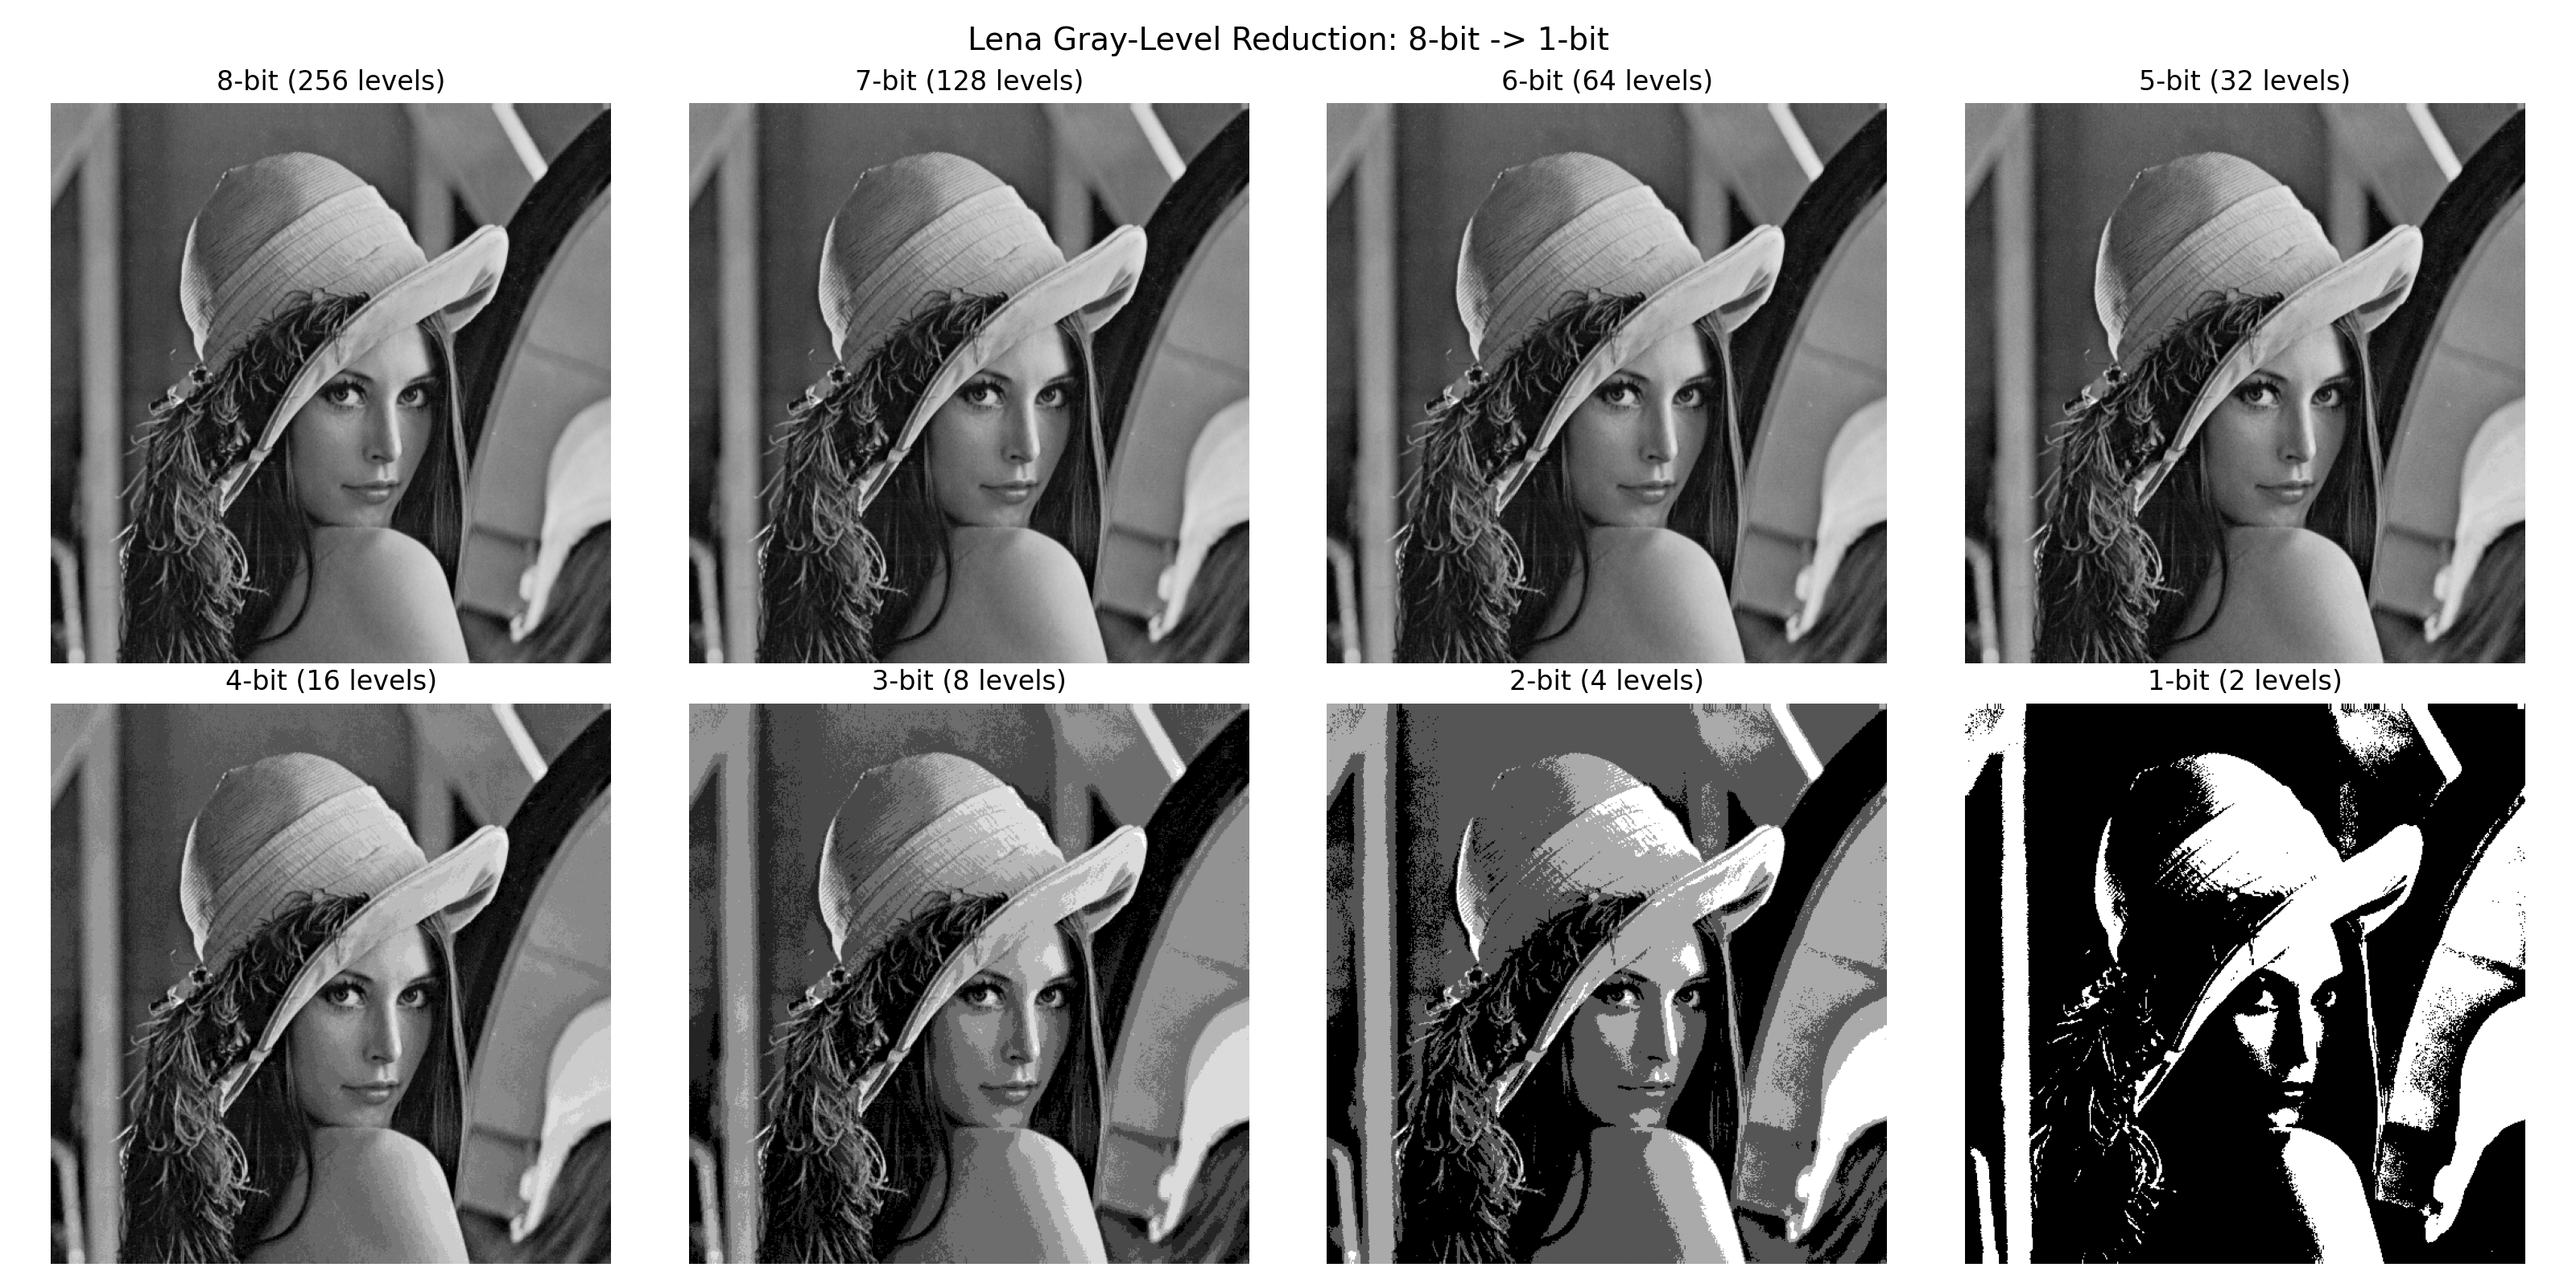
\includegraphics[width=0.92\textwidth]{task2_gray_levels_overview.png}
  \caption{Lena 灰度级递减总览（8 bit $\rightarrow$ 1 bit）}
\end{figure}

分析：位深降低后，灰度层次减少，伪轮廓（banding）逐渐明显。1 bit 时仅保留黑白两级，纹理细节损失最明显。

\subsection{任务3：Lena 均值和方差}
\begin{table}[H]
\centering
\caption{Lena 灰度统计结果}
\begin{tabular}{lc}
\toprule
统计量 & 数值 \\
\midrule
Mean & 99.051216 \\
Variance & 2796.031839 \\
\bottomrule
\end{tabular}
\end{table}

结果表明图像整体亮度偏中低灰，且灰度分布具有一定离散度，存在较丰富亮暗变化。

\subsection{任务4：三种插值放大到 $2048\times2048$}
\begin{figure}[H]
  \centering
  \begin{subfigure}{0.32\textwidth}
    \centering
    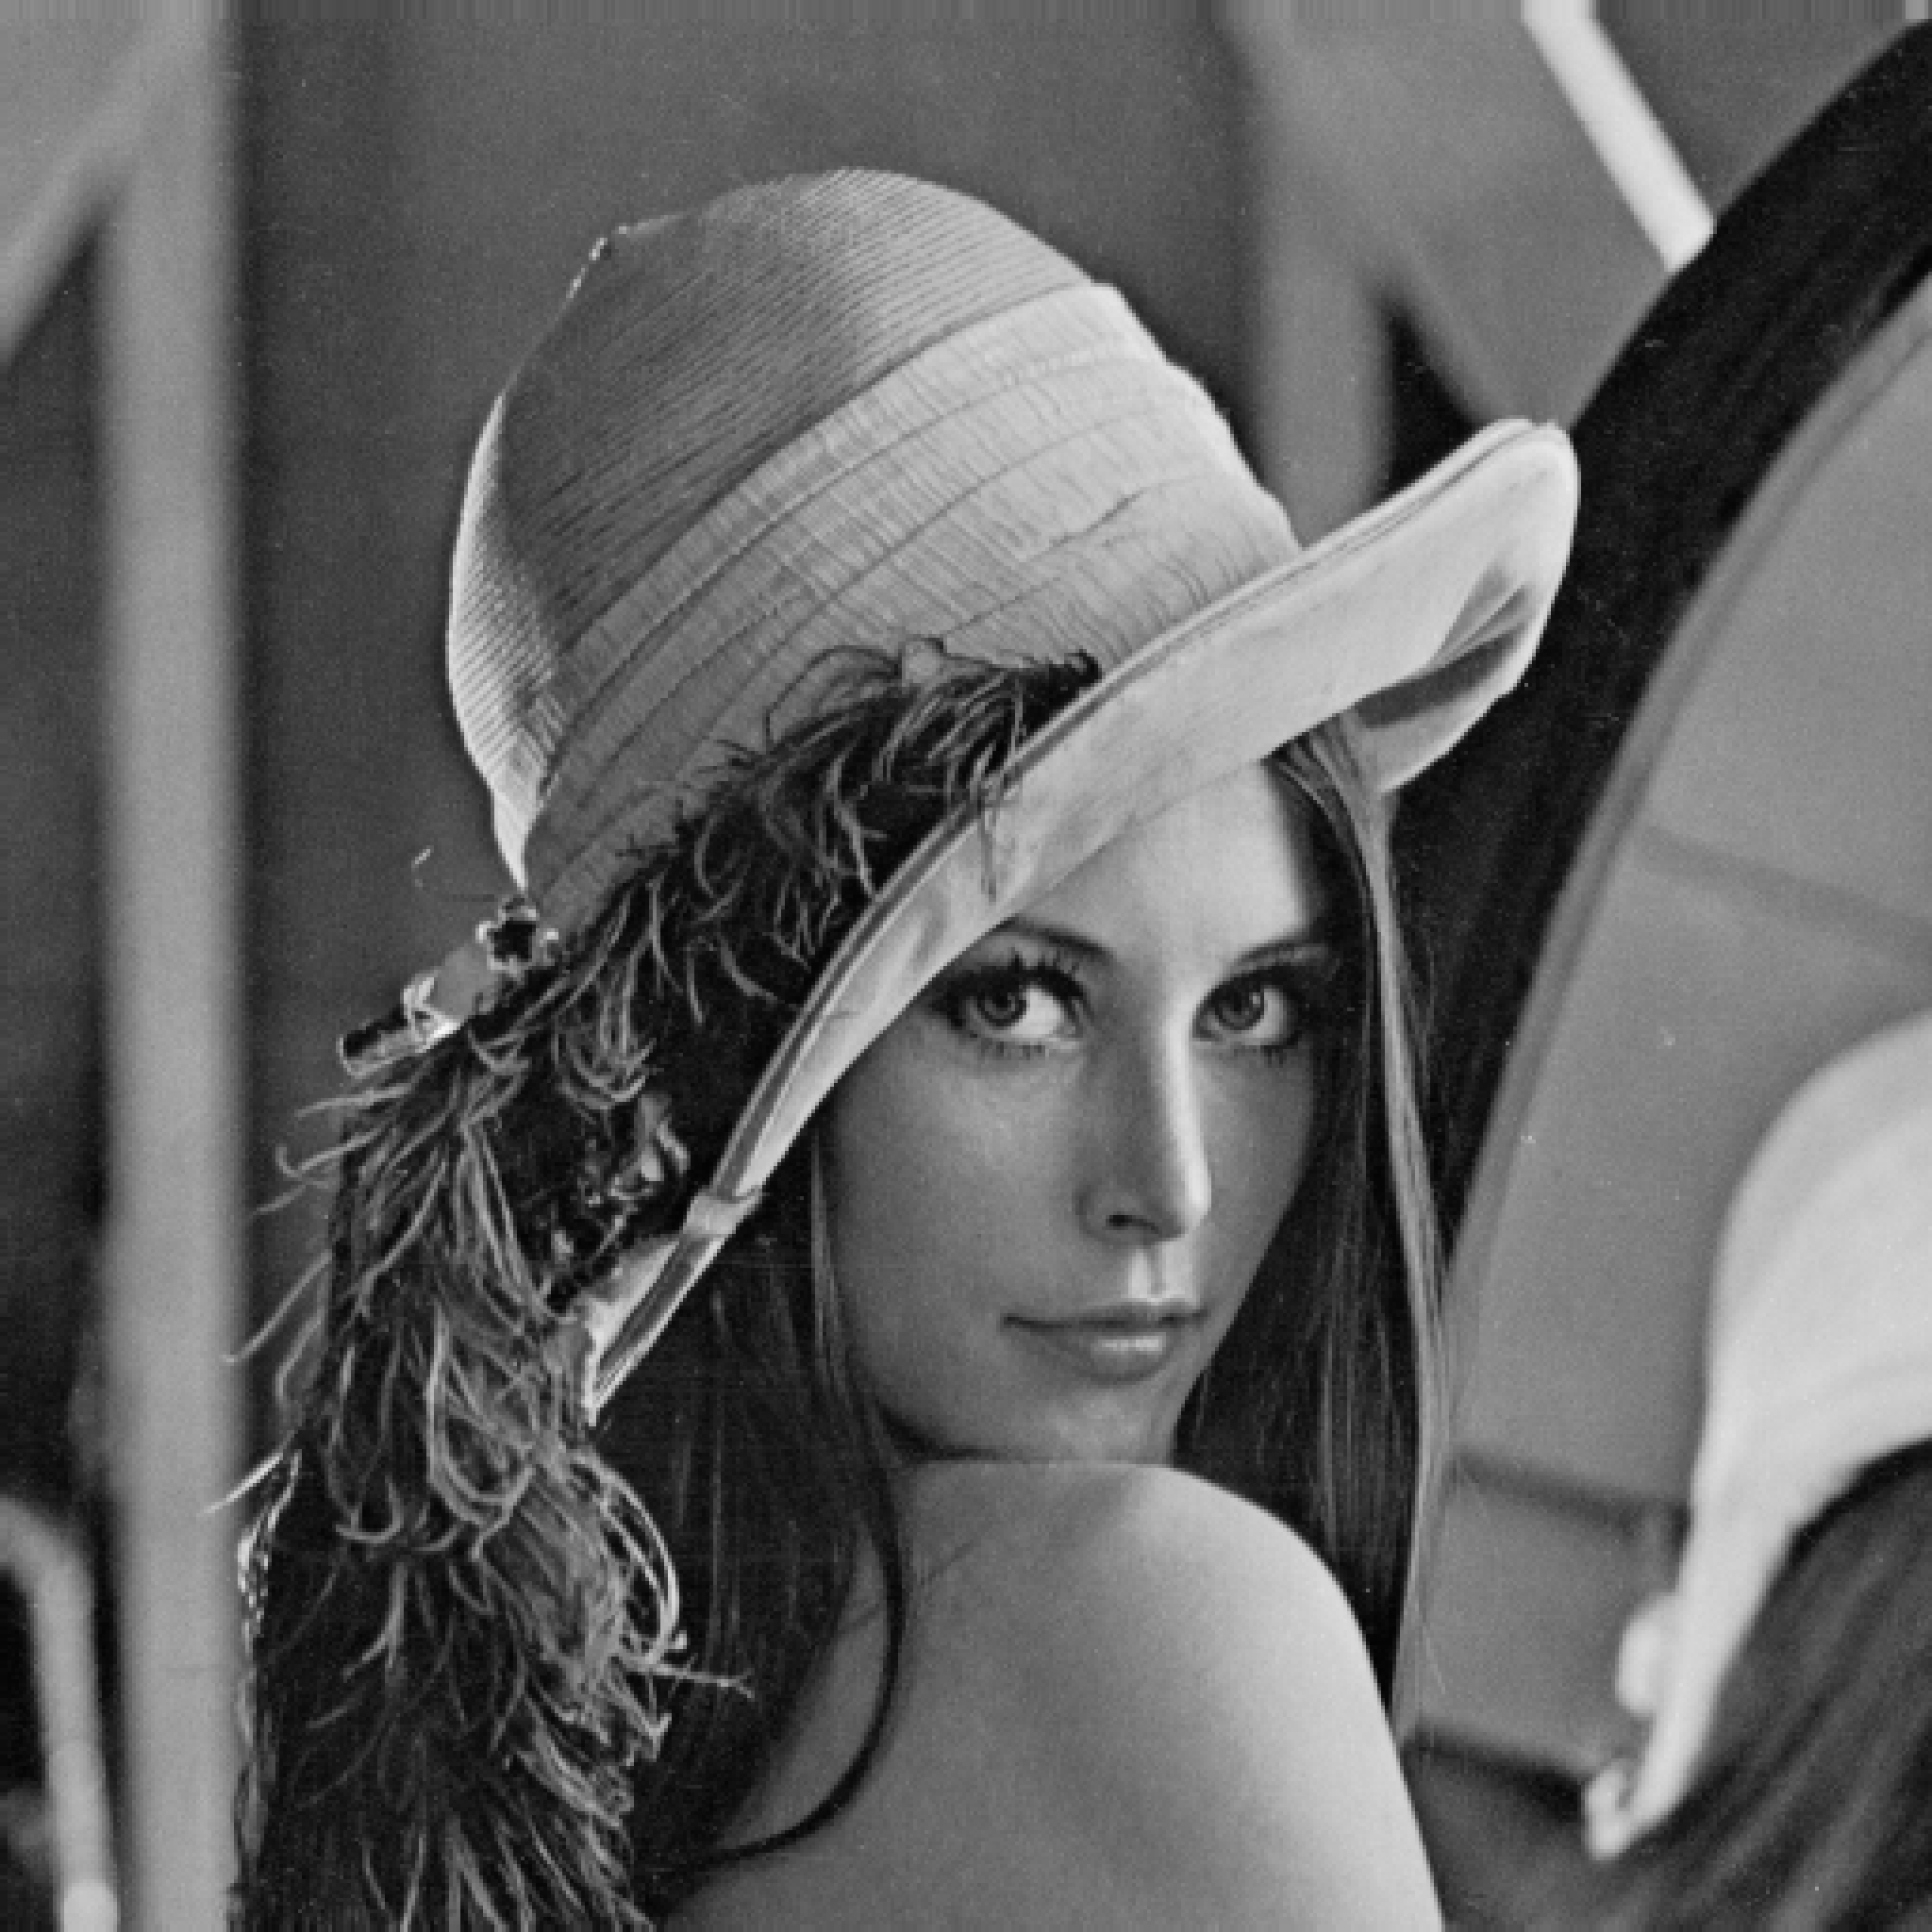
\includegraphics[width=\linewidth]{lena_2048_nearest.png}
    \caption{Nearest}
  \end{subfigure}
  \begin{subfigure}{0.32\textwidth}
    \centering
    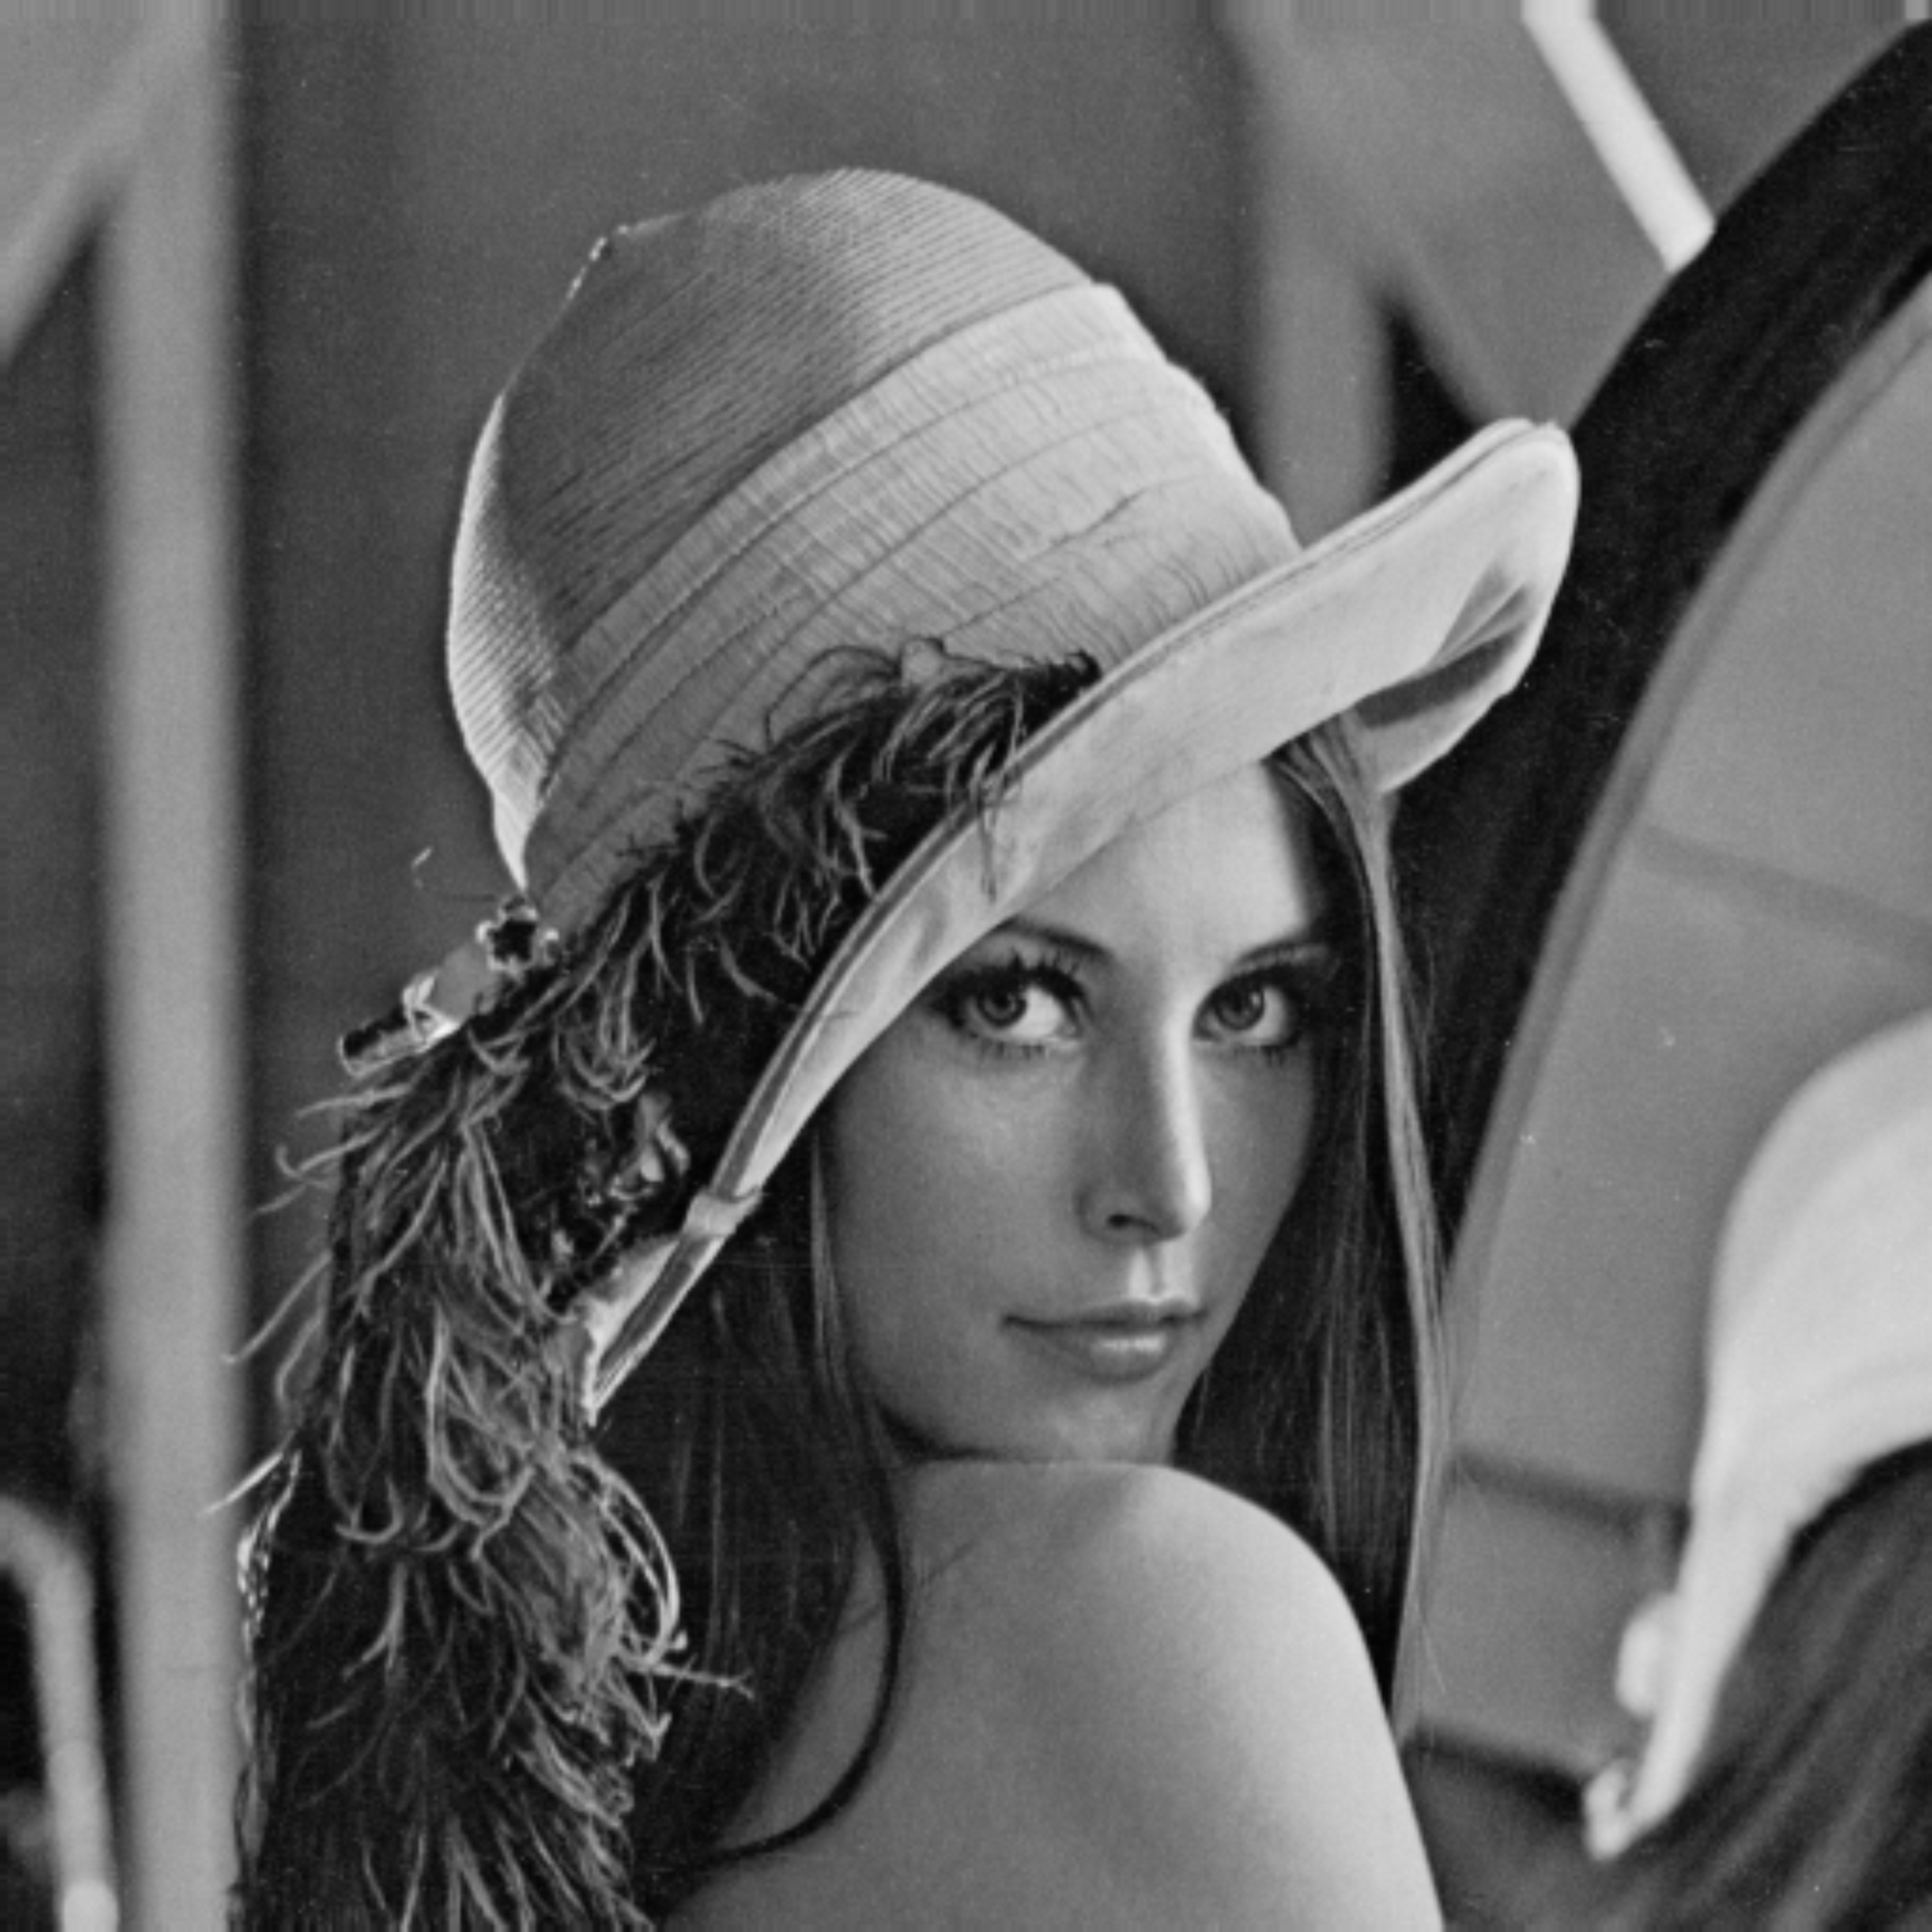
\includegraphics[width=\linewidth]{lena_2048_bilinear.png}
    \caption{Bilinear}
  \end{subfigure}
  \begin{subfigure}{0.32\textwidth}
    \centering
    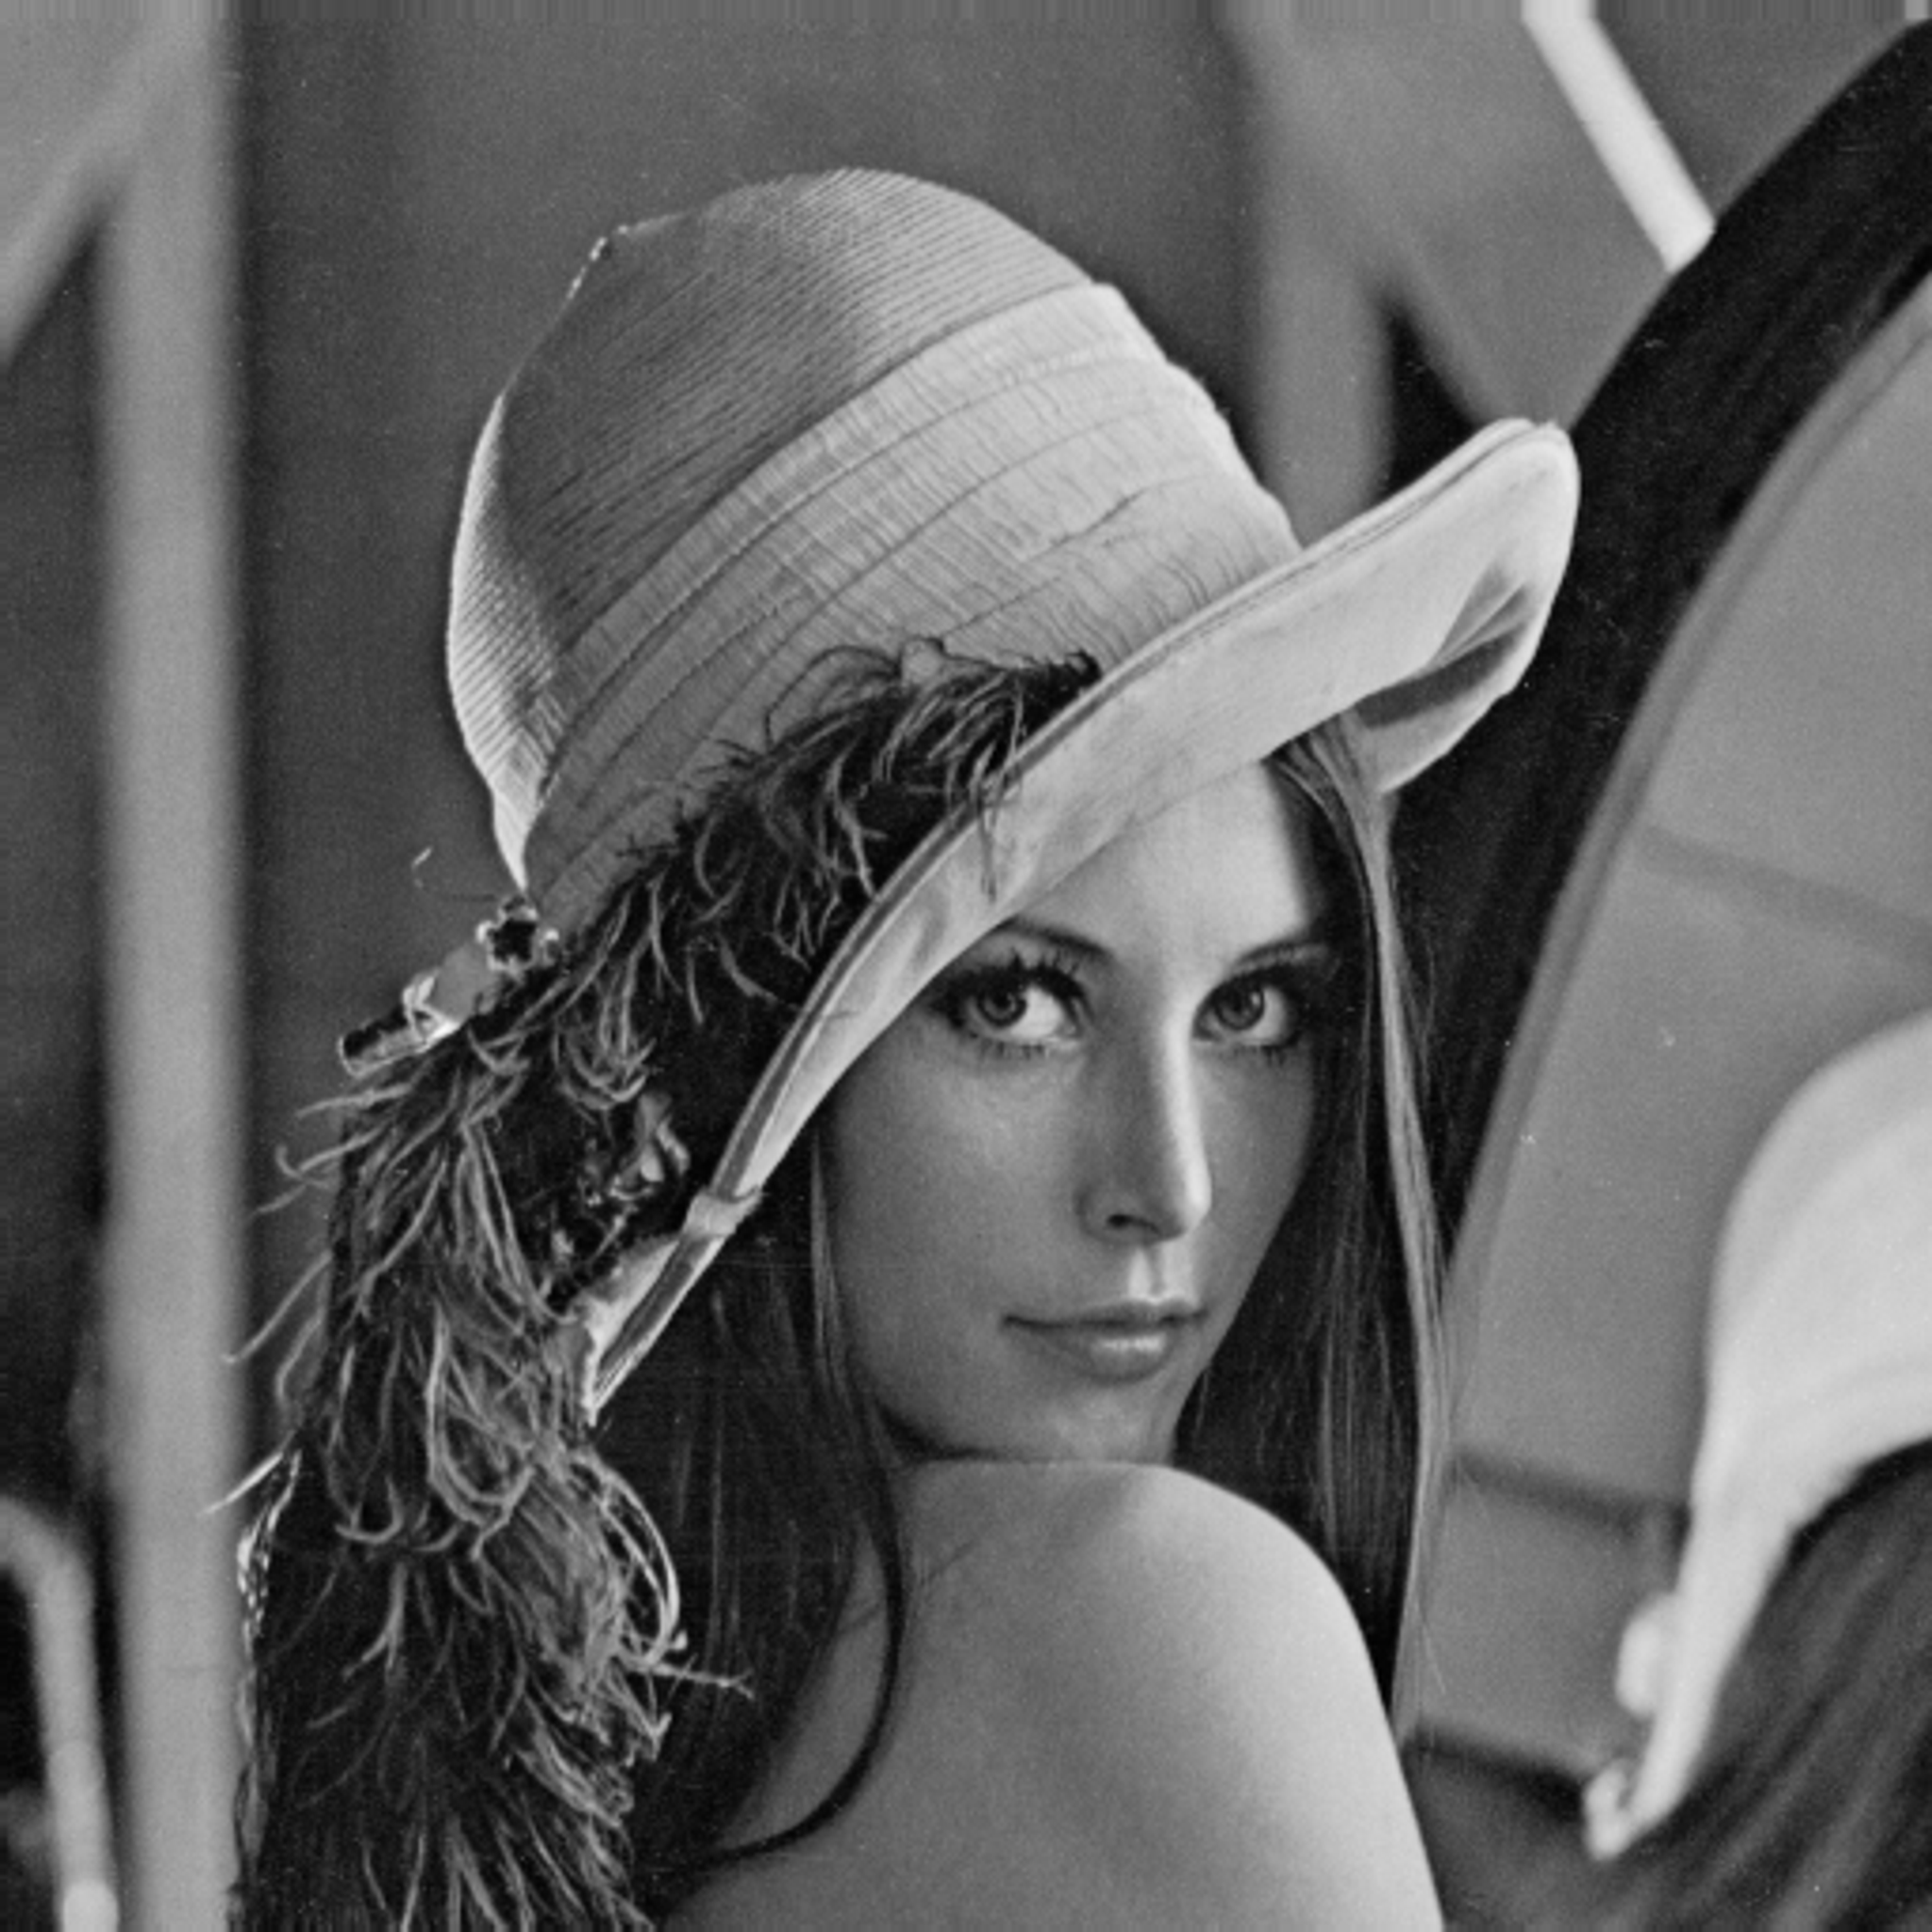
\includegraphics[width=\linewidth]{lena_2048_bicubic.png}
    \caption{Bicubic}
  \end{subfigure}
  \caption{Lena 三种插值放大效果对比}
\end{figure}

分析：近邻插值锯齿与块效应最明显；双线性更平滑但边缘稍软；双三次在平滑与锐度之间表现更均衡。

\subsection{任务5：几何变换 + 三插值放大}
\subsubsection*{(1) 变换中间结果}
\begin{figure}[H]
  \centering
  \begin{subfigure}{0.48\textwidth}
    \centering
    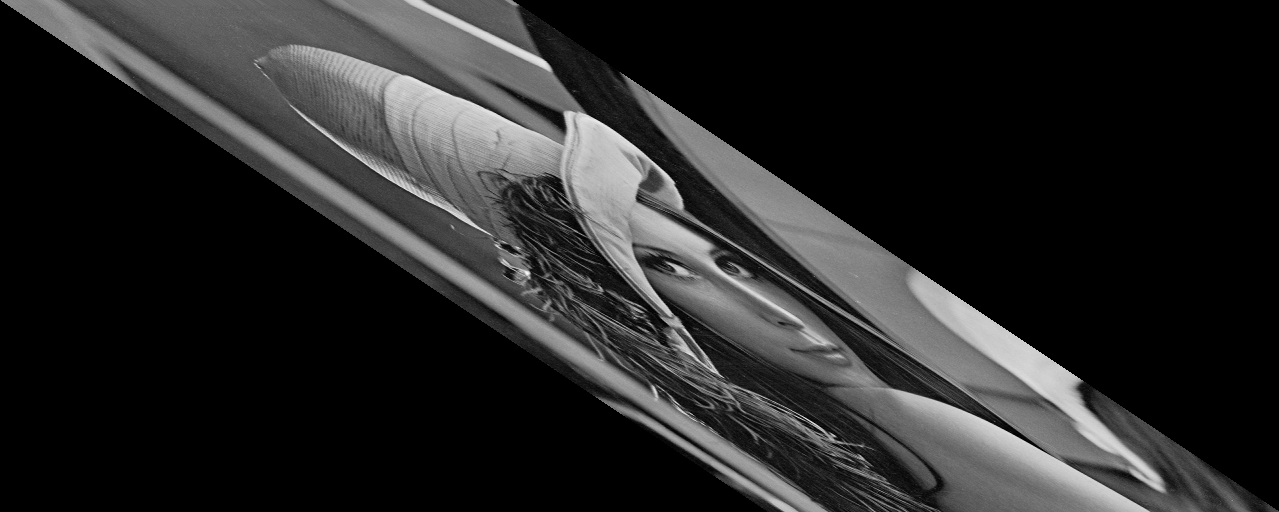
\includegraphics[width=\linewidth]{lena_shear_k1.5.png}
    \caption{Lena: Shear($k=1.5$)}
  \end{subfigure}
  \begin{subfigure}{0.48\textwidth}
    \centering
    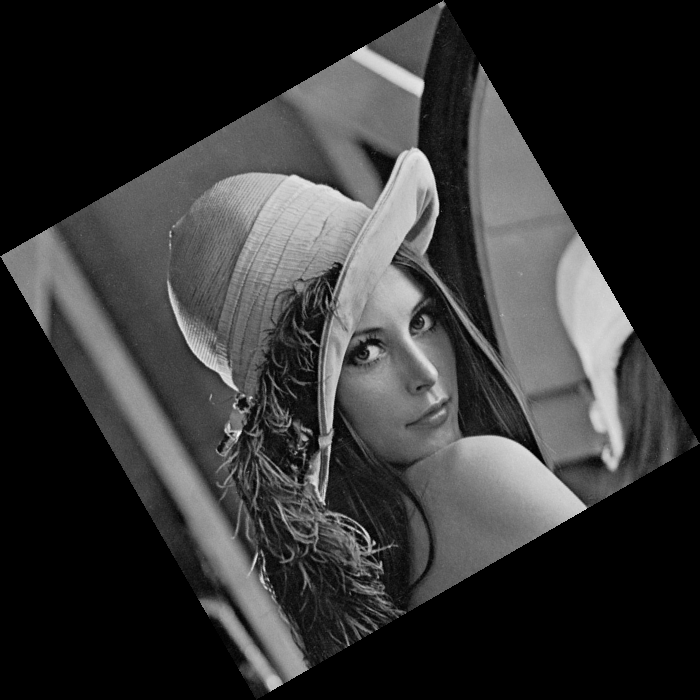
\includegraphics[width=\linewidth]{lena_rotate_30deg.png}
    \caption{Lena: Rotate($30^\circ$)}
  \end{subfigure}

  \vspace{0.5em}
  \begin{subfigure}{0.48\textwidth}
    \centering
    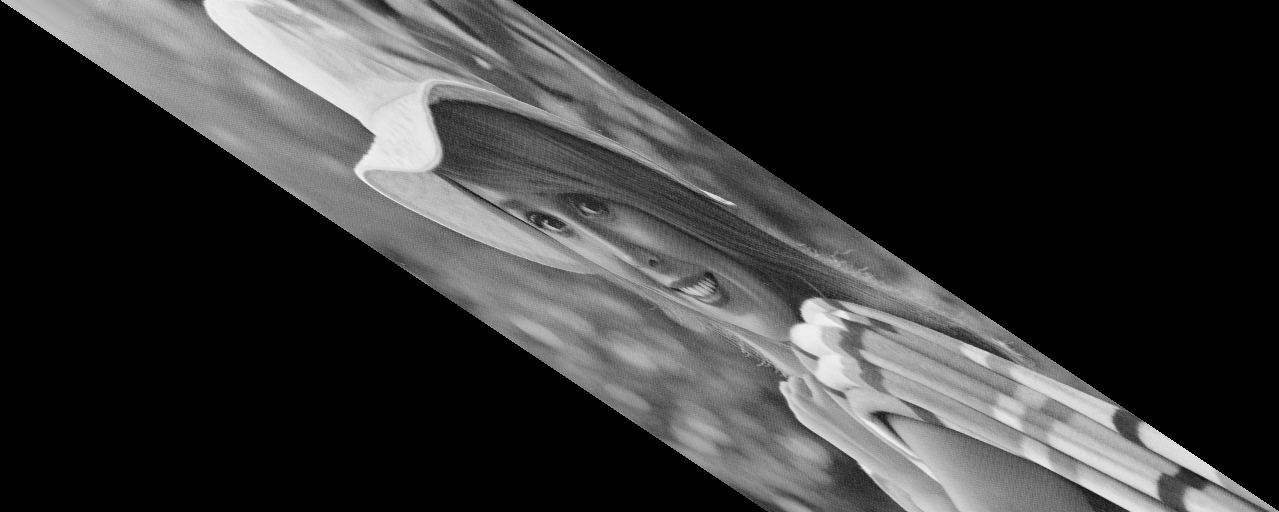
\includegraphics[width=\linewidth]{elain1_shear_k1.5.png}
    \caption{Elain1: Shear($k=1.5$)}
  \end{subfigure}
  \begin{subfigure}{0.48\textwidth}
    \centering
    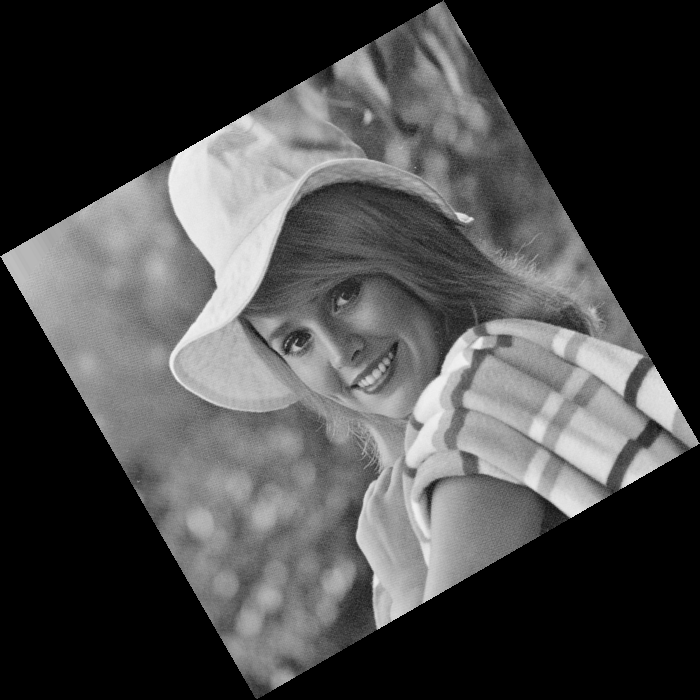
\includegraphics[width=\linewidth]{elain1_rotate_30deg.png}
    \caption{Elain1: Rotate($30^\circ$)}
  \end{subfigure}
  \caption{Lena 与 Elain1 的几何变换中间结果}
\end{figure}

其中 Lena 原图为 $512\times512$，shear 后尺寸为 $1279\times512$，旋转后尺寸为 $700\times700$。

\subsubsection*{(2) Lena：Shear 后插值放大}
\begin{figure}[H]
  \centering
  \begin{subfigure}{0.32\textwidth}
    \centering
    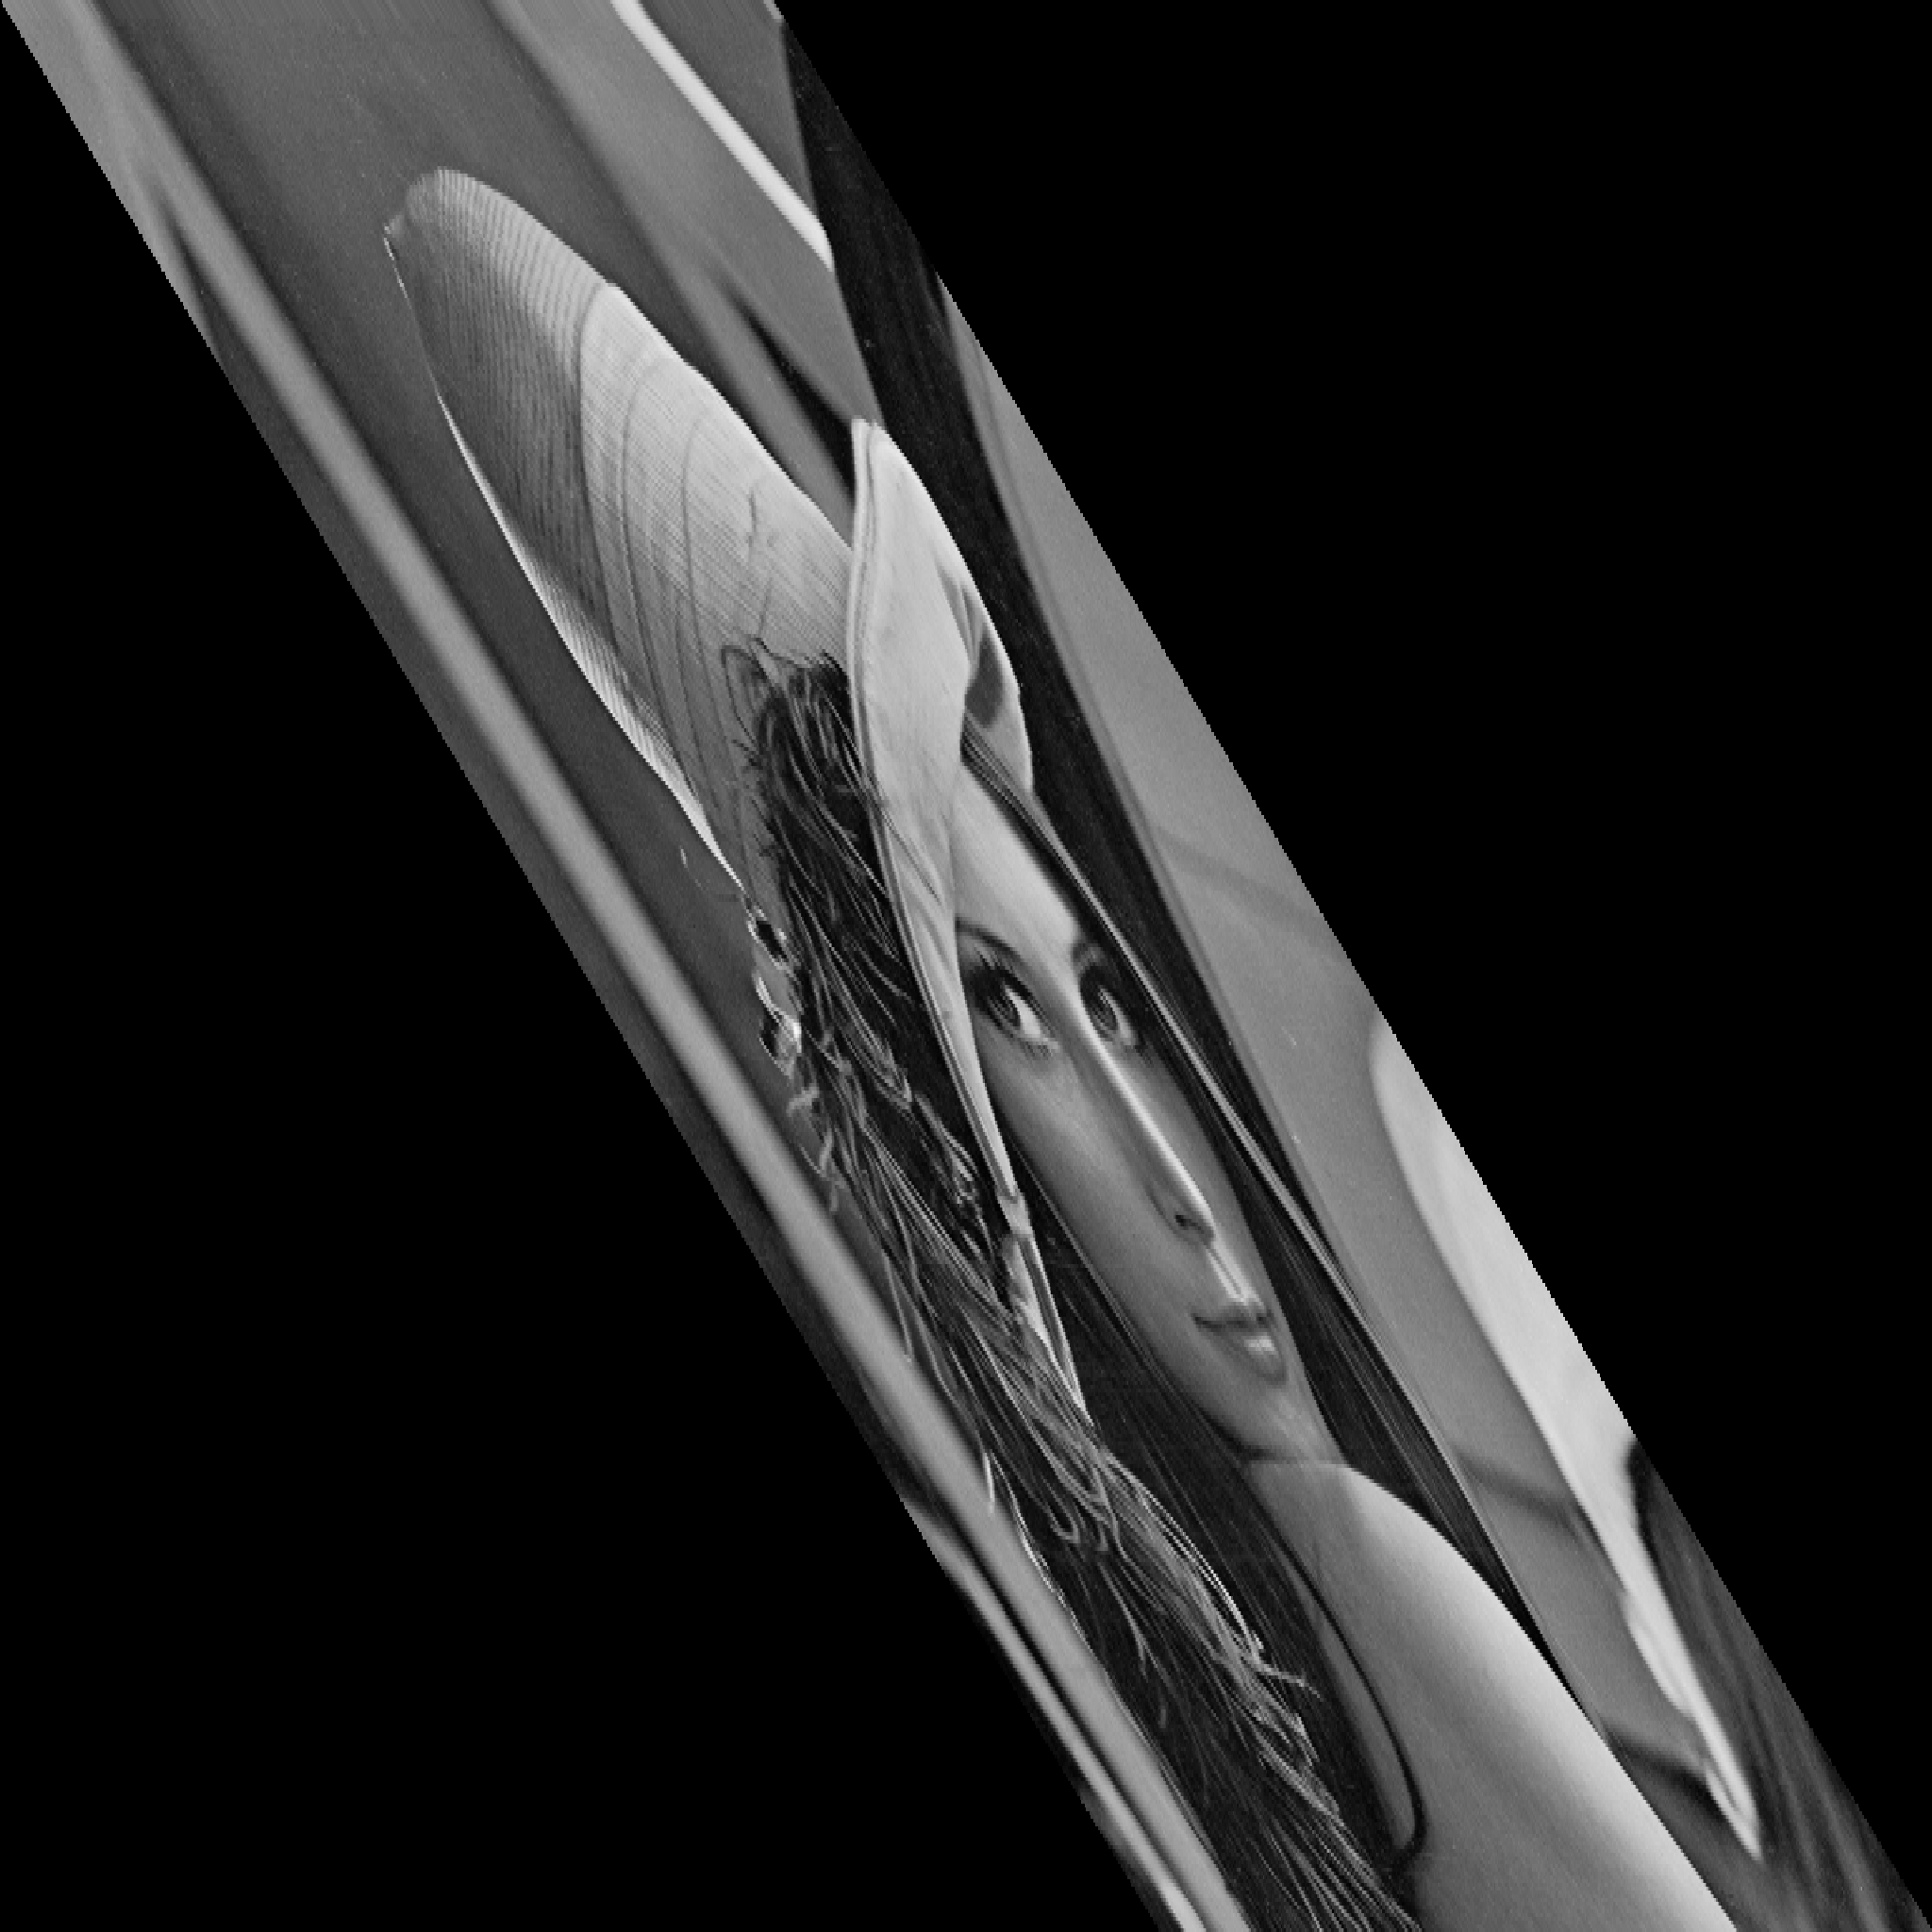
\includegraphics[width=\linewidth]{lena_shear_k1.5_2048_nearest.png}
    \caption{Nearest}
  \end{subfigure}
  \begin{subfigure}{0.32\textwidth}
    \centering
    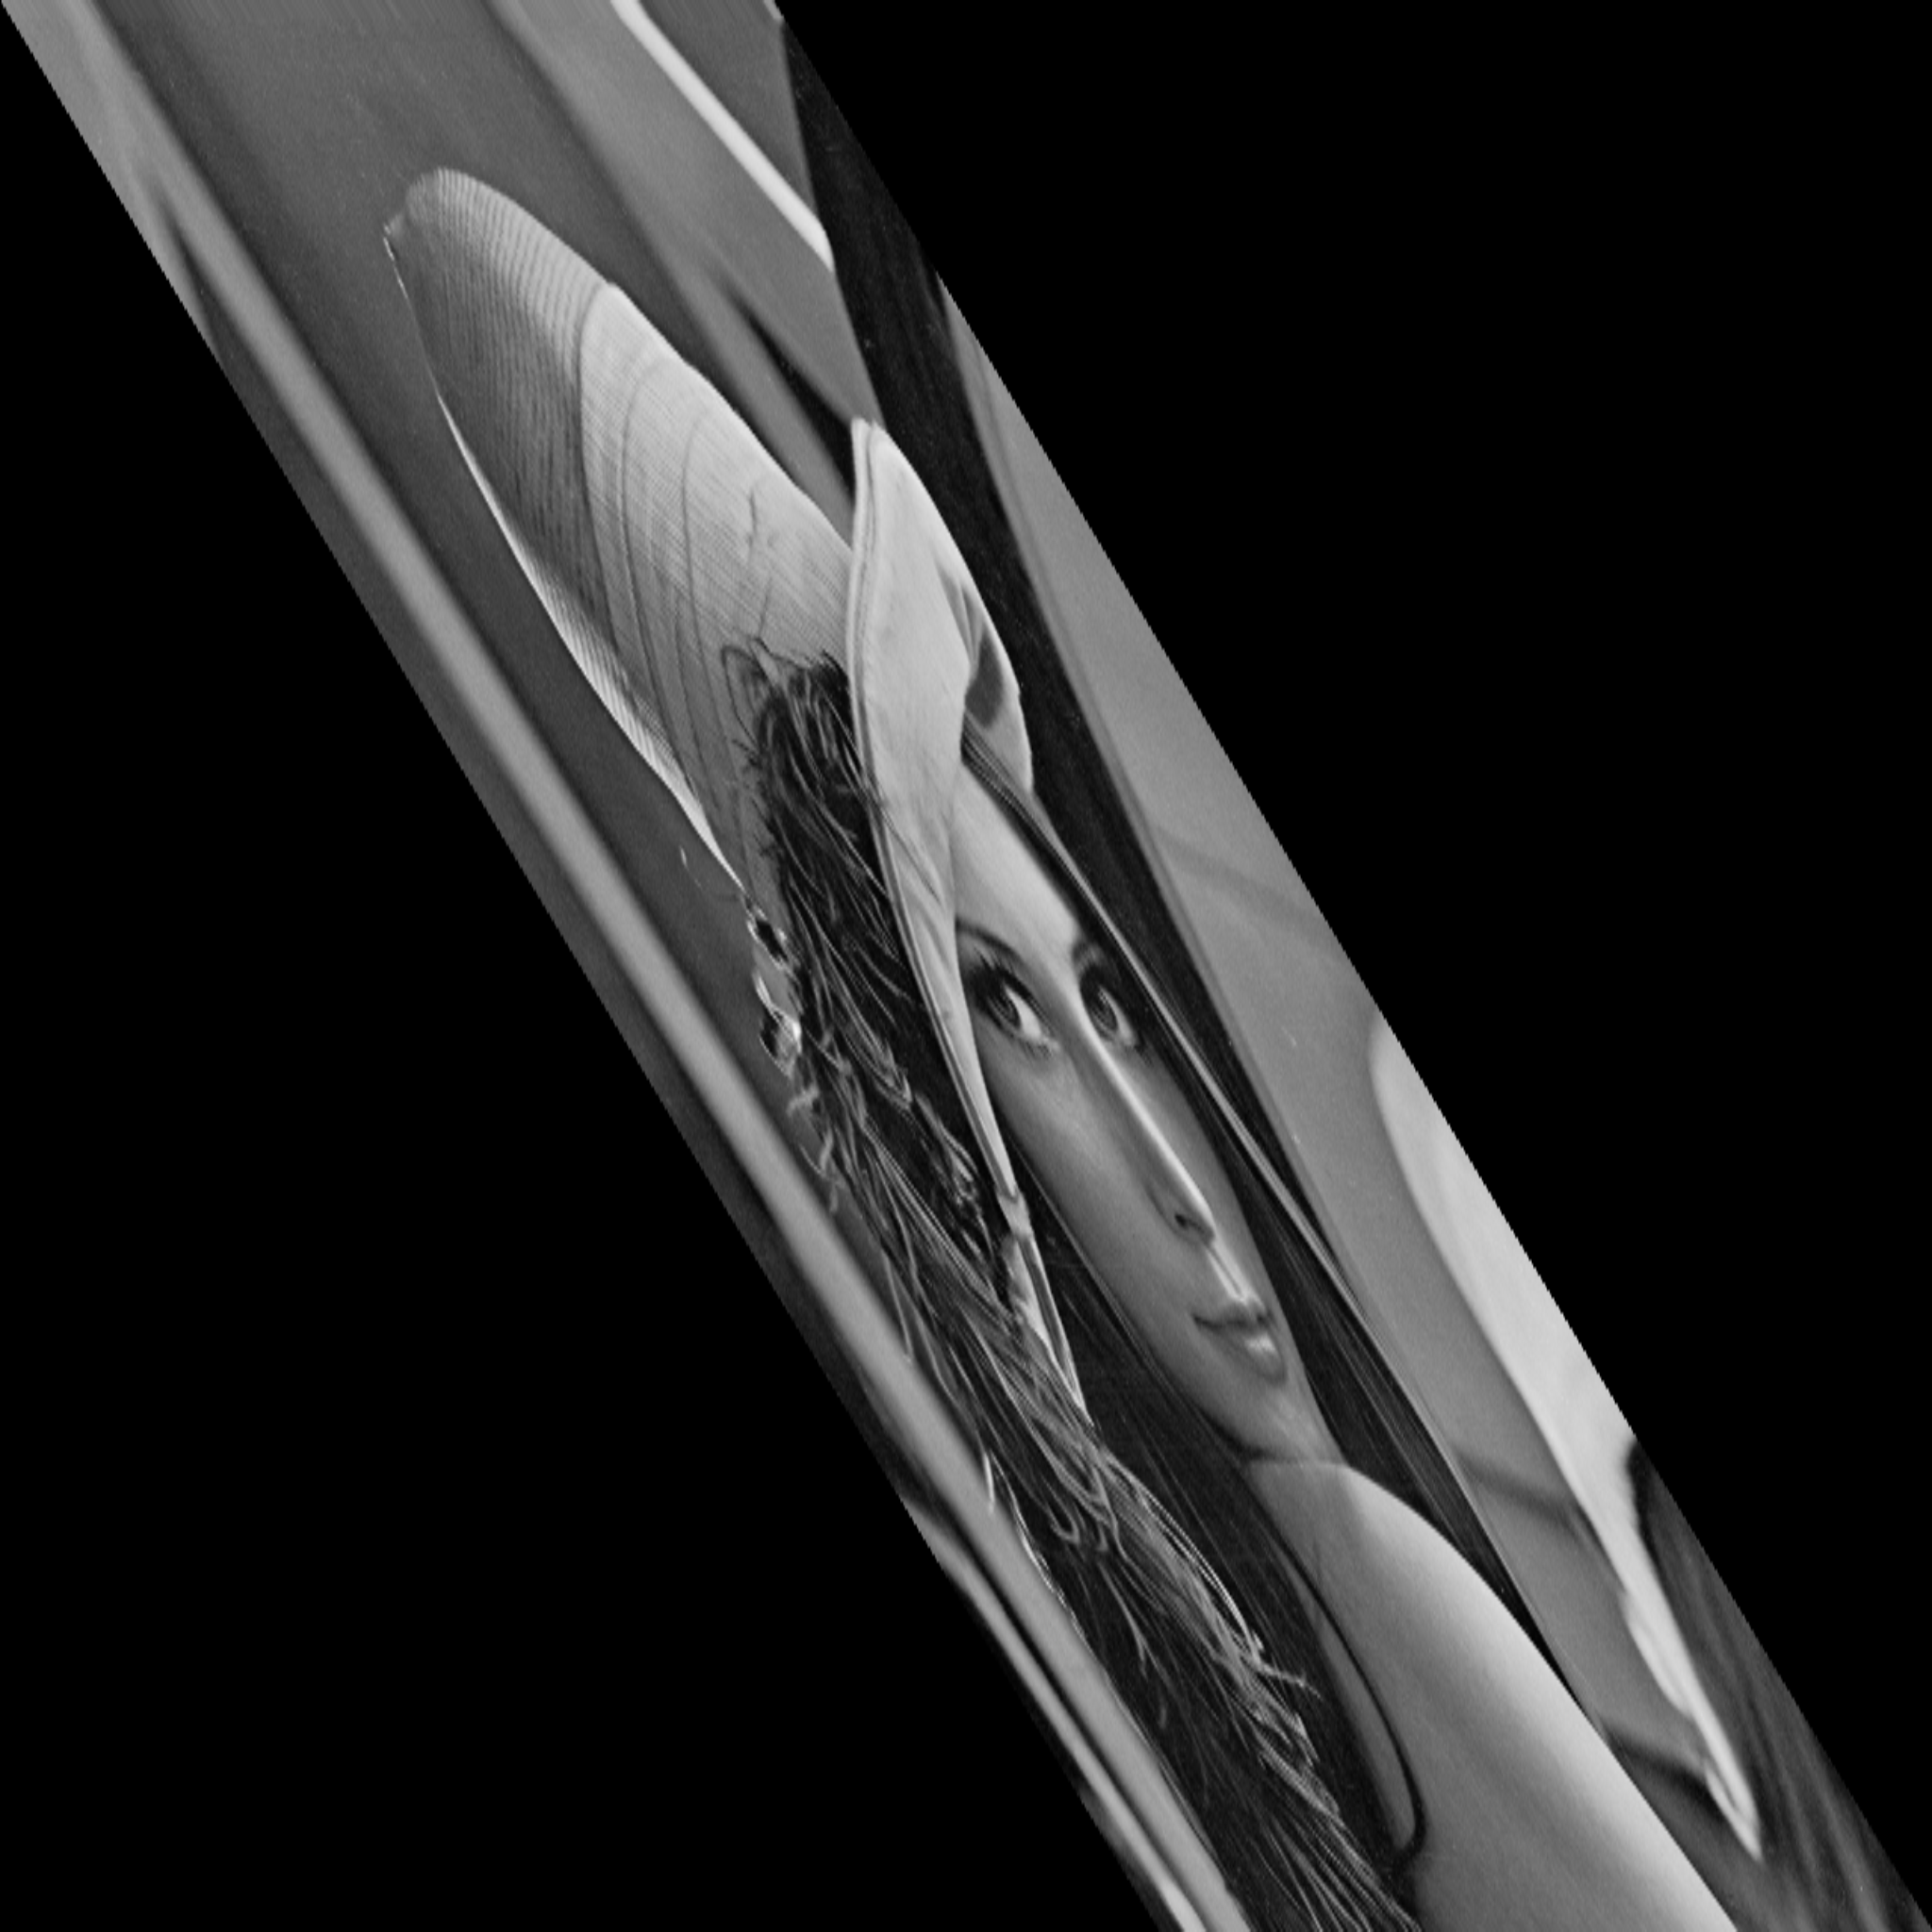
\includegraphics[width=\linewidth]{lena_shear_k1.5_2048_bilinear.png}
    \caption{Bilinear}
  \end{subfigure}
  \begin{subfigure}{0.32\textwidth}
    \centering
    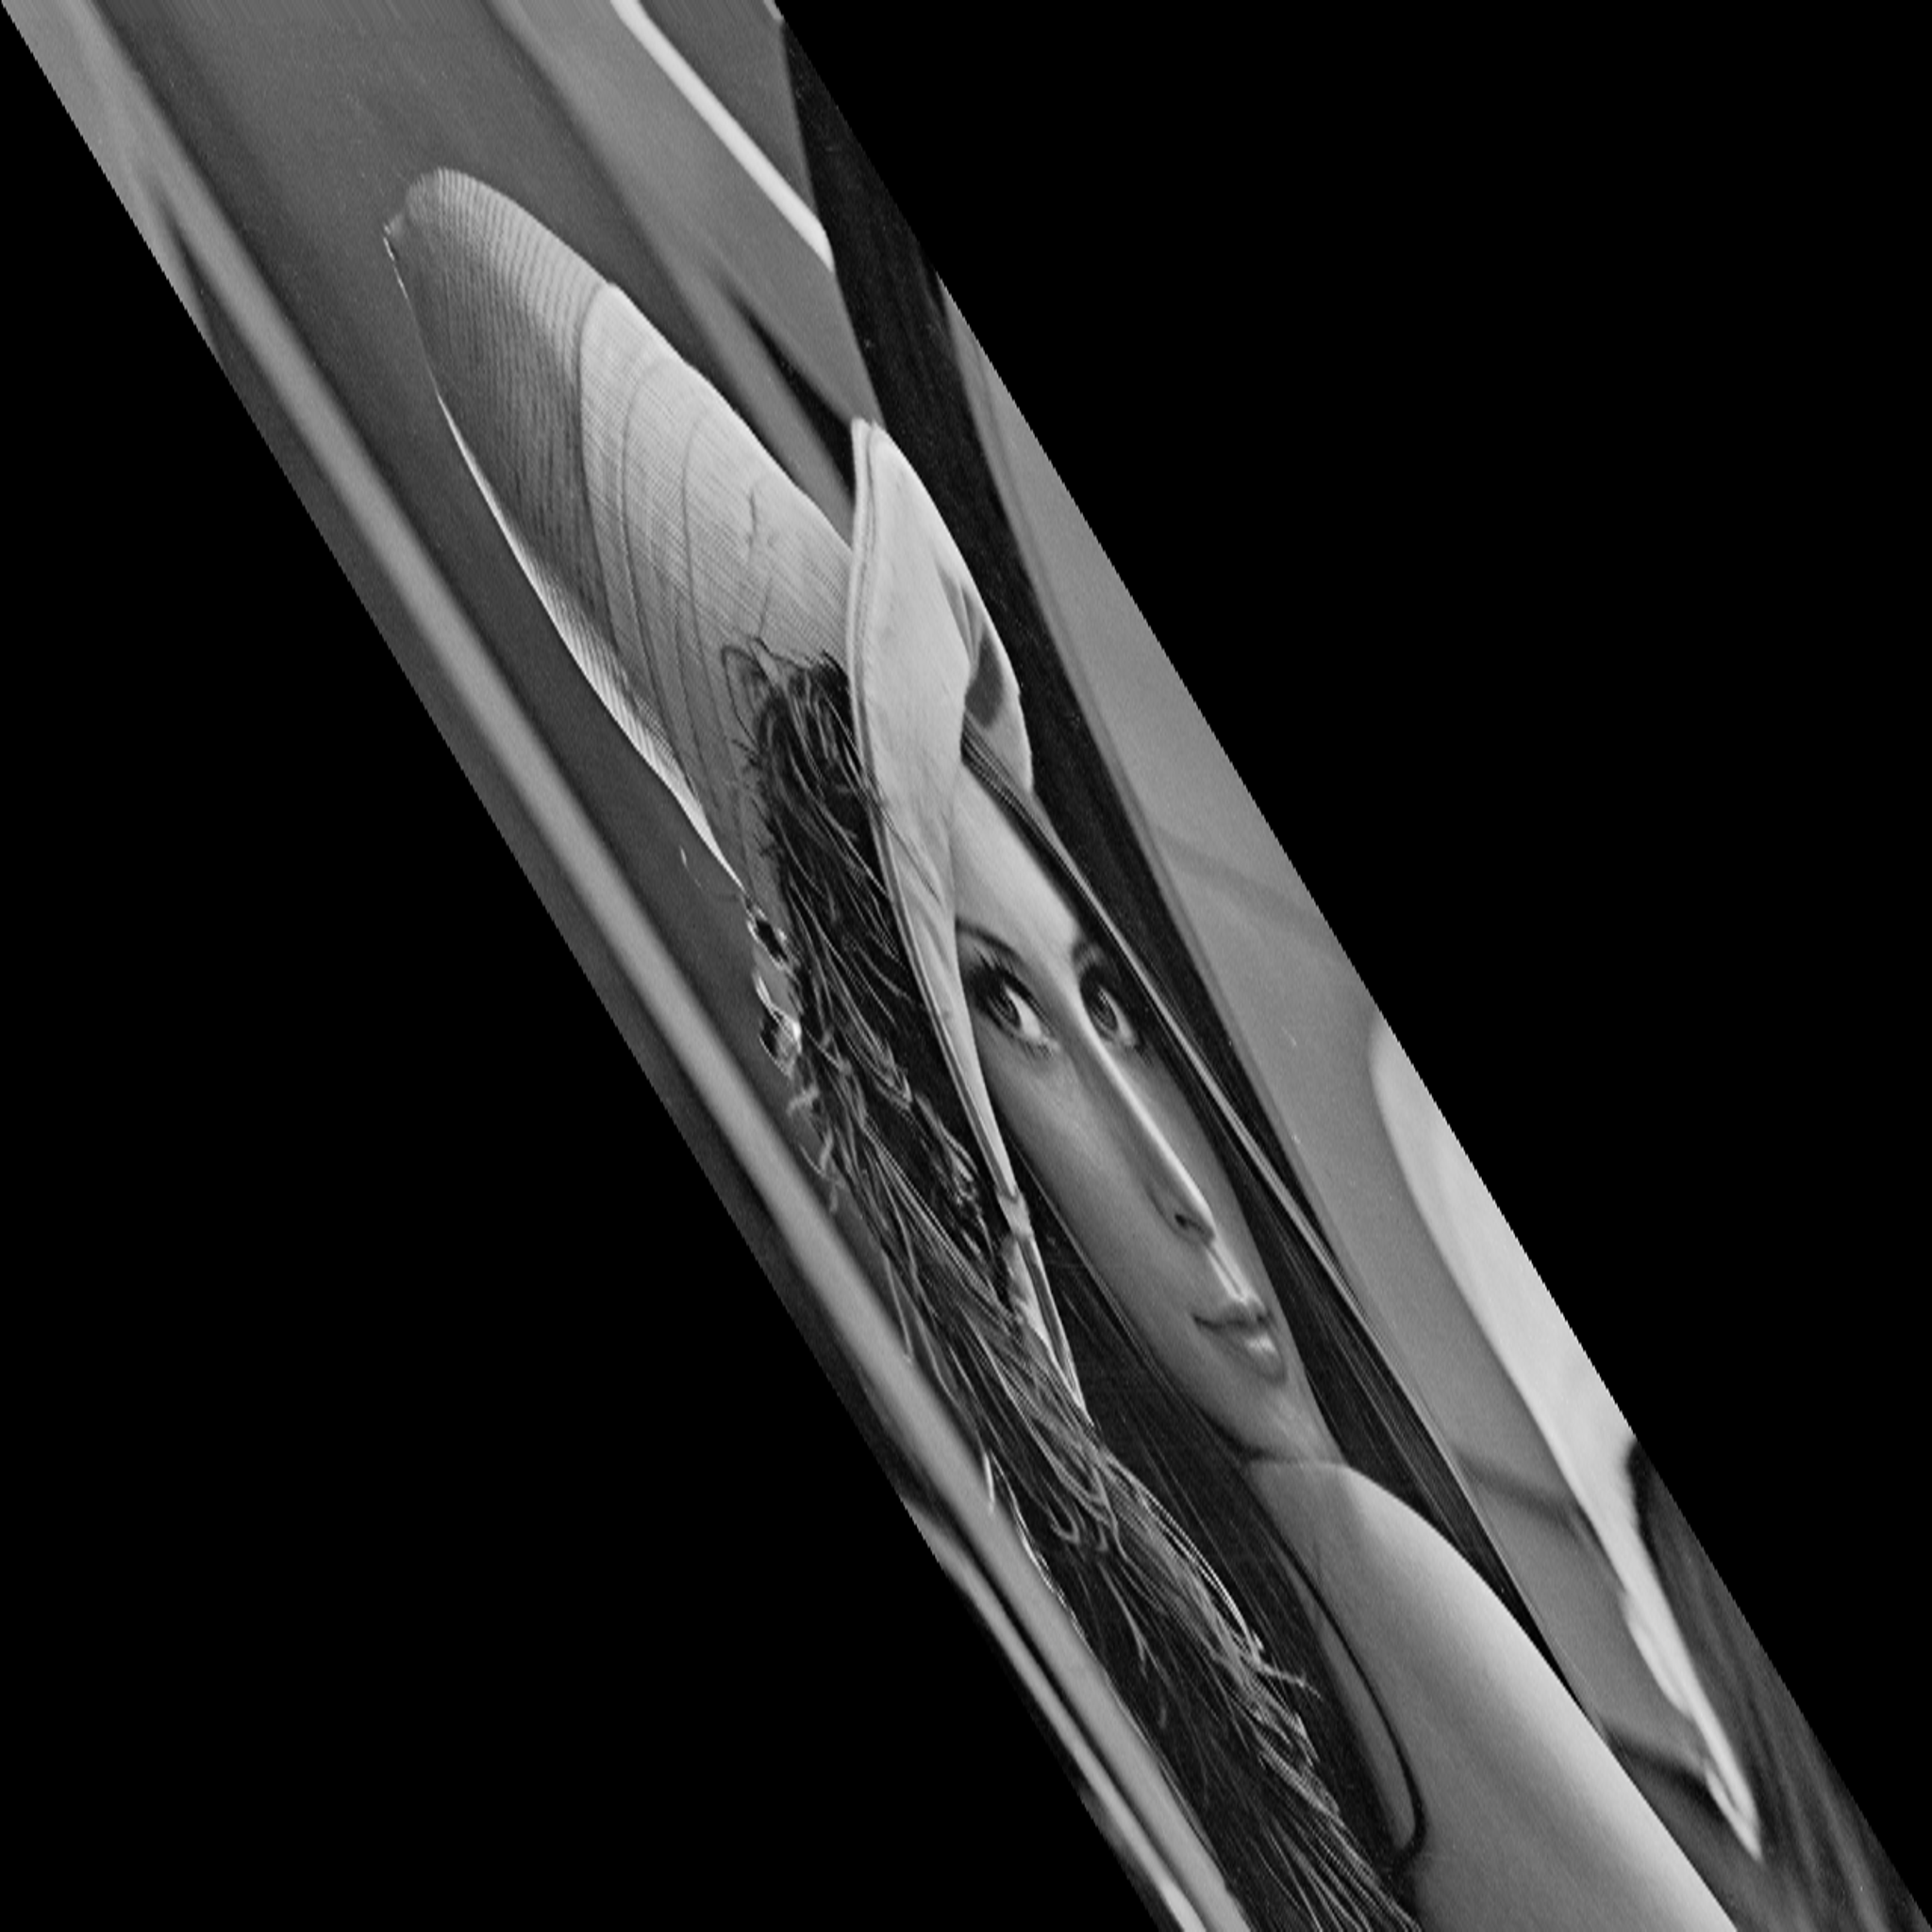
\includegraphics[width=\linewidth]{lena_shear_k1.5_2048_bicubic.png}
    \caption{Bicubic}
  \end{subfigure}
  \caption{Lena Shear 后三种插值放大对比}
\end{figure}

\subsubsection*{(3) Lena：旋转后插值放大}
\begin{figure}[H]
  \centering
  \begin{subfigure}{0.32\textwidth}
    \centering
    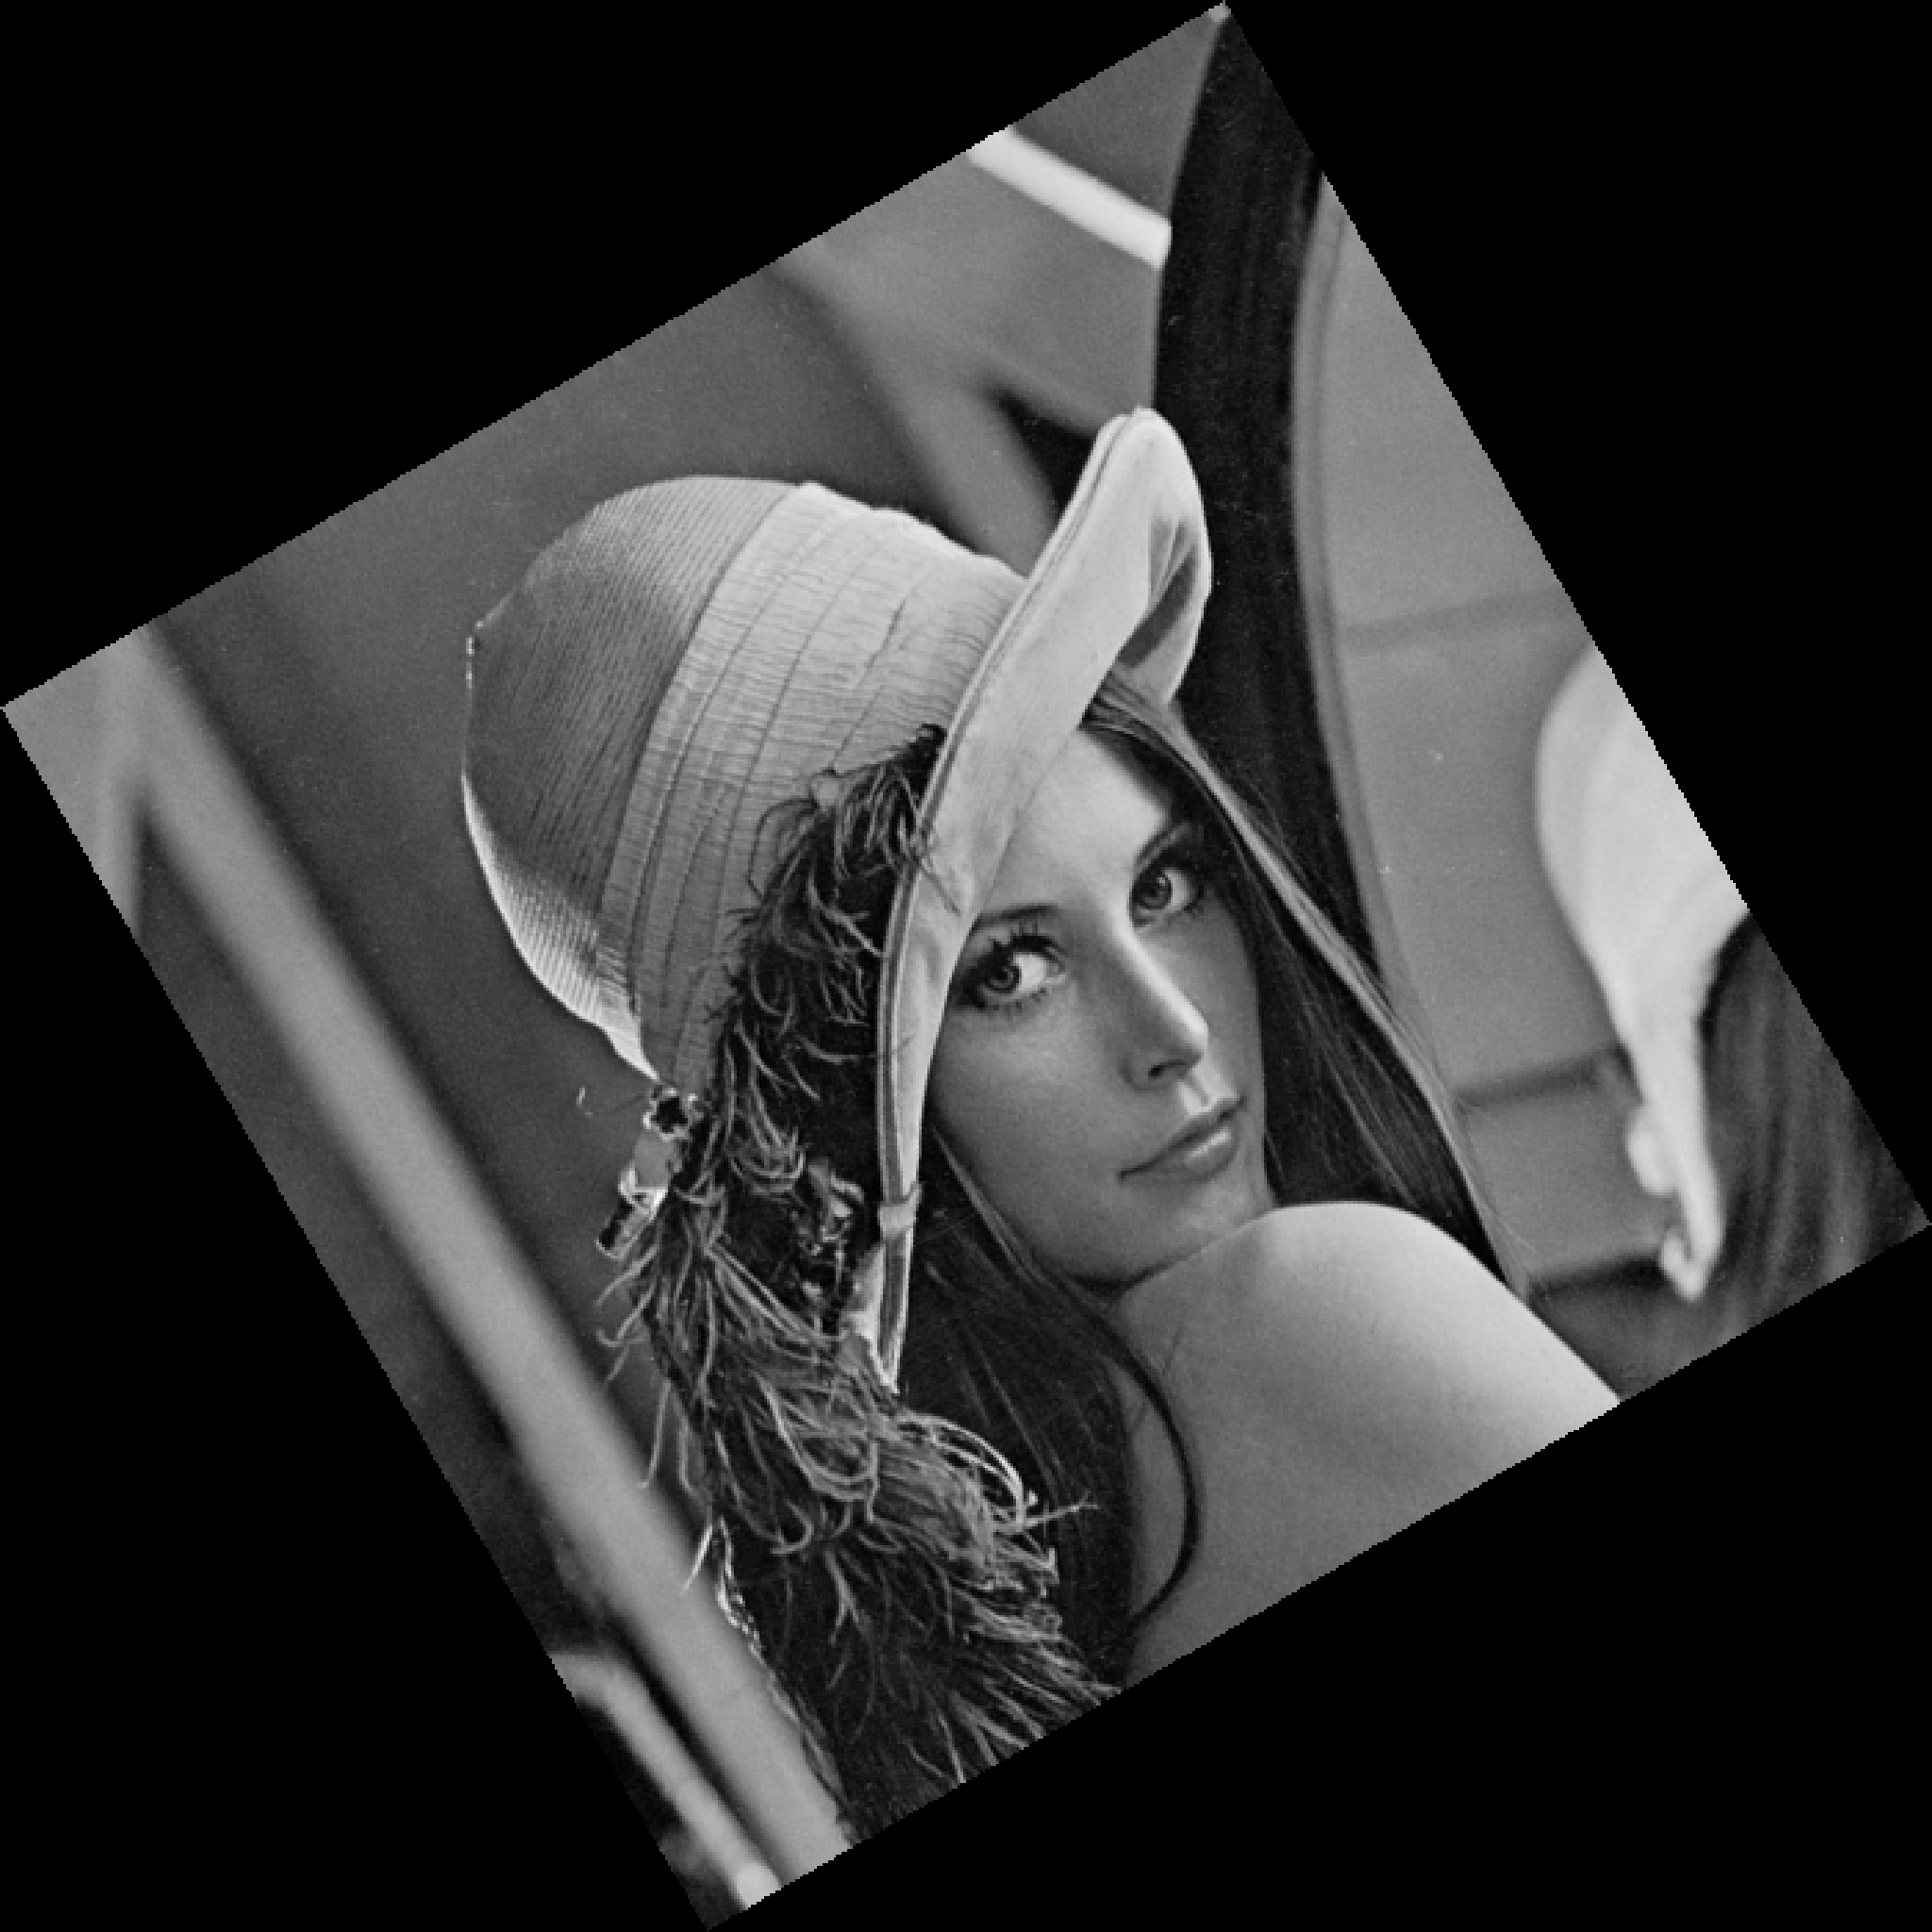
\includegraphics[width=\linewidth]{lena_rotate_30deg_2048_nearest.png}
    \caption{Nearest}
  \end{subfigure}
  \begin{subfigure}{0.32\textwidth}
    \centering
    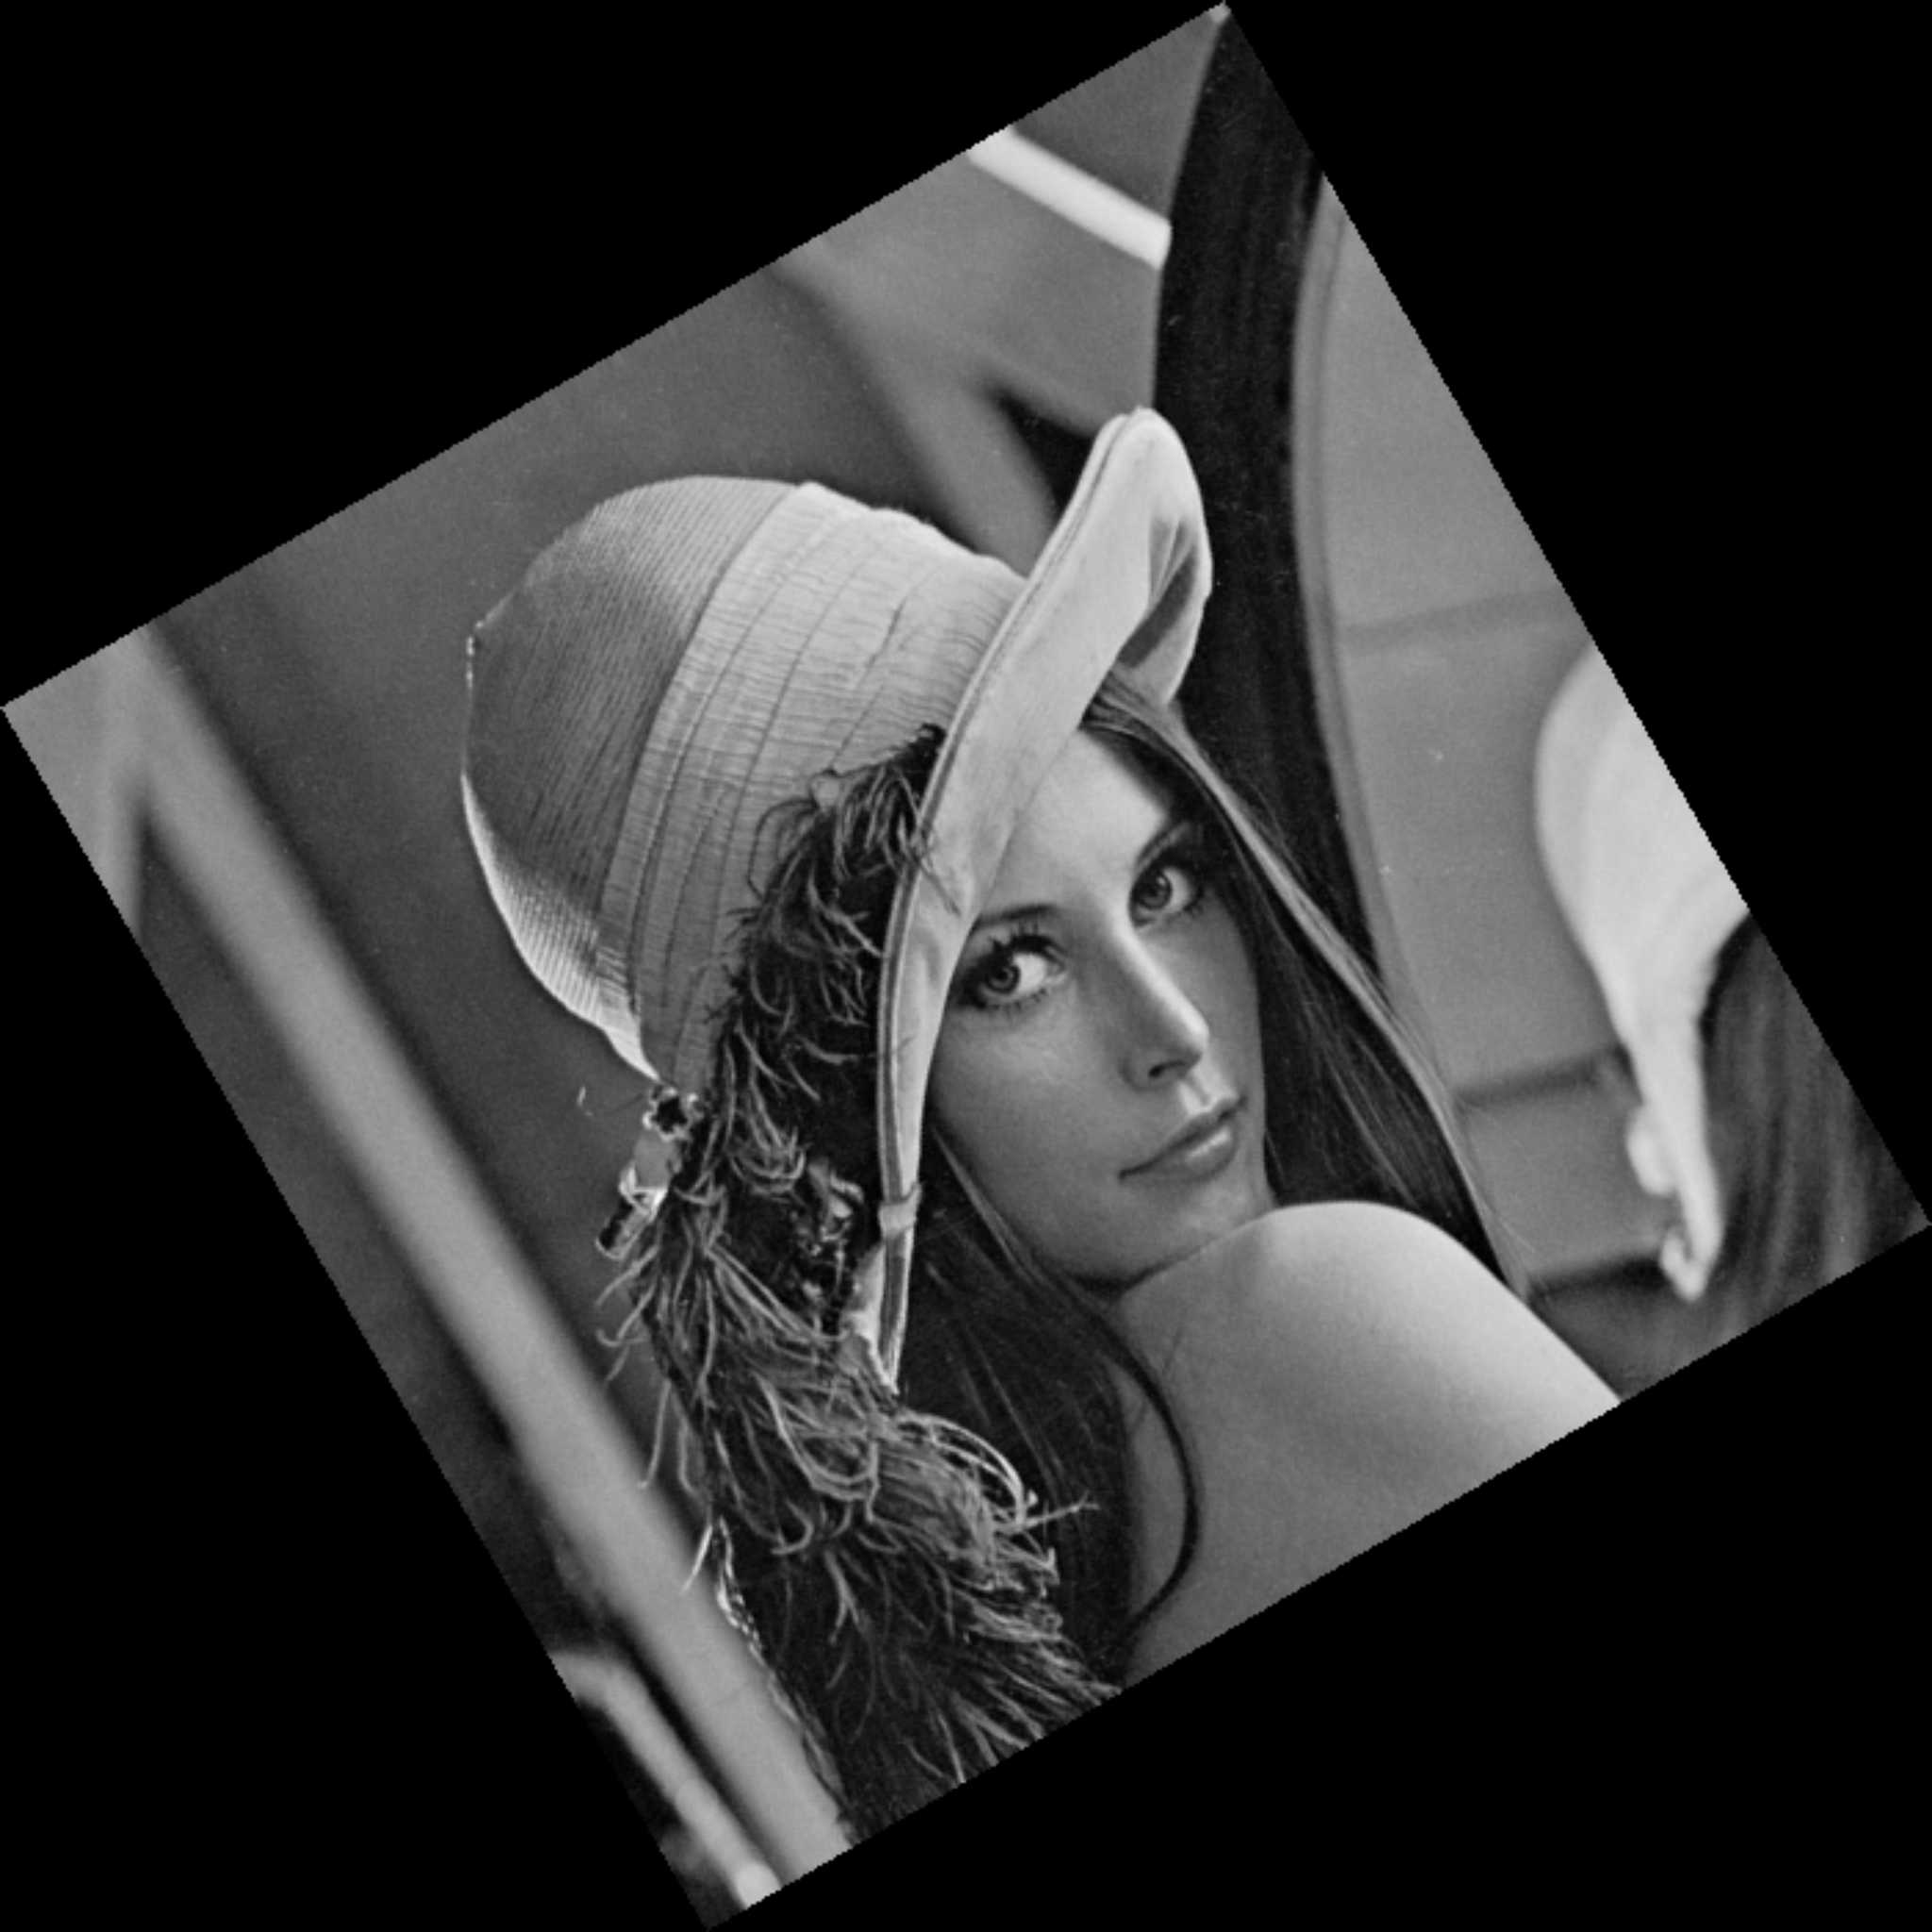
\includegraphics[width=\linewidth]{lena_rotate_30deg_2048_bilinear.png}
    \caption{Bilinear}
  \end{subfigure}
  \begin{subfigure}{0.32\textwidth}
    \centering
    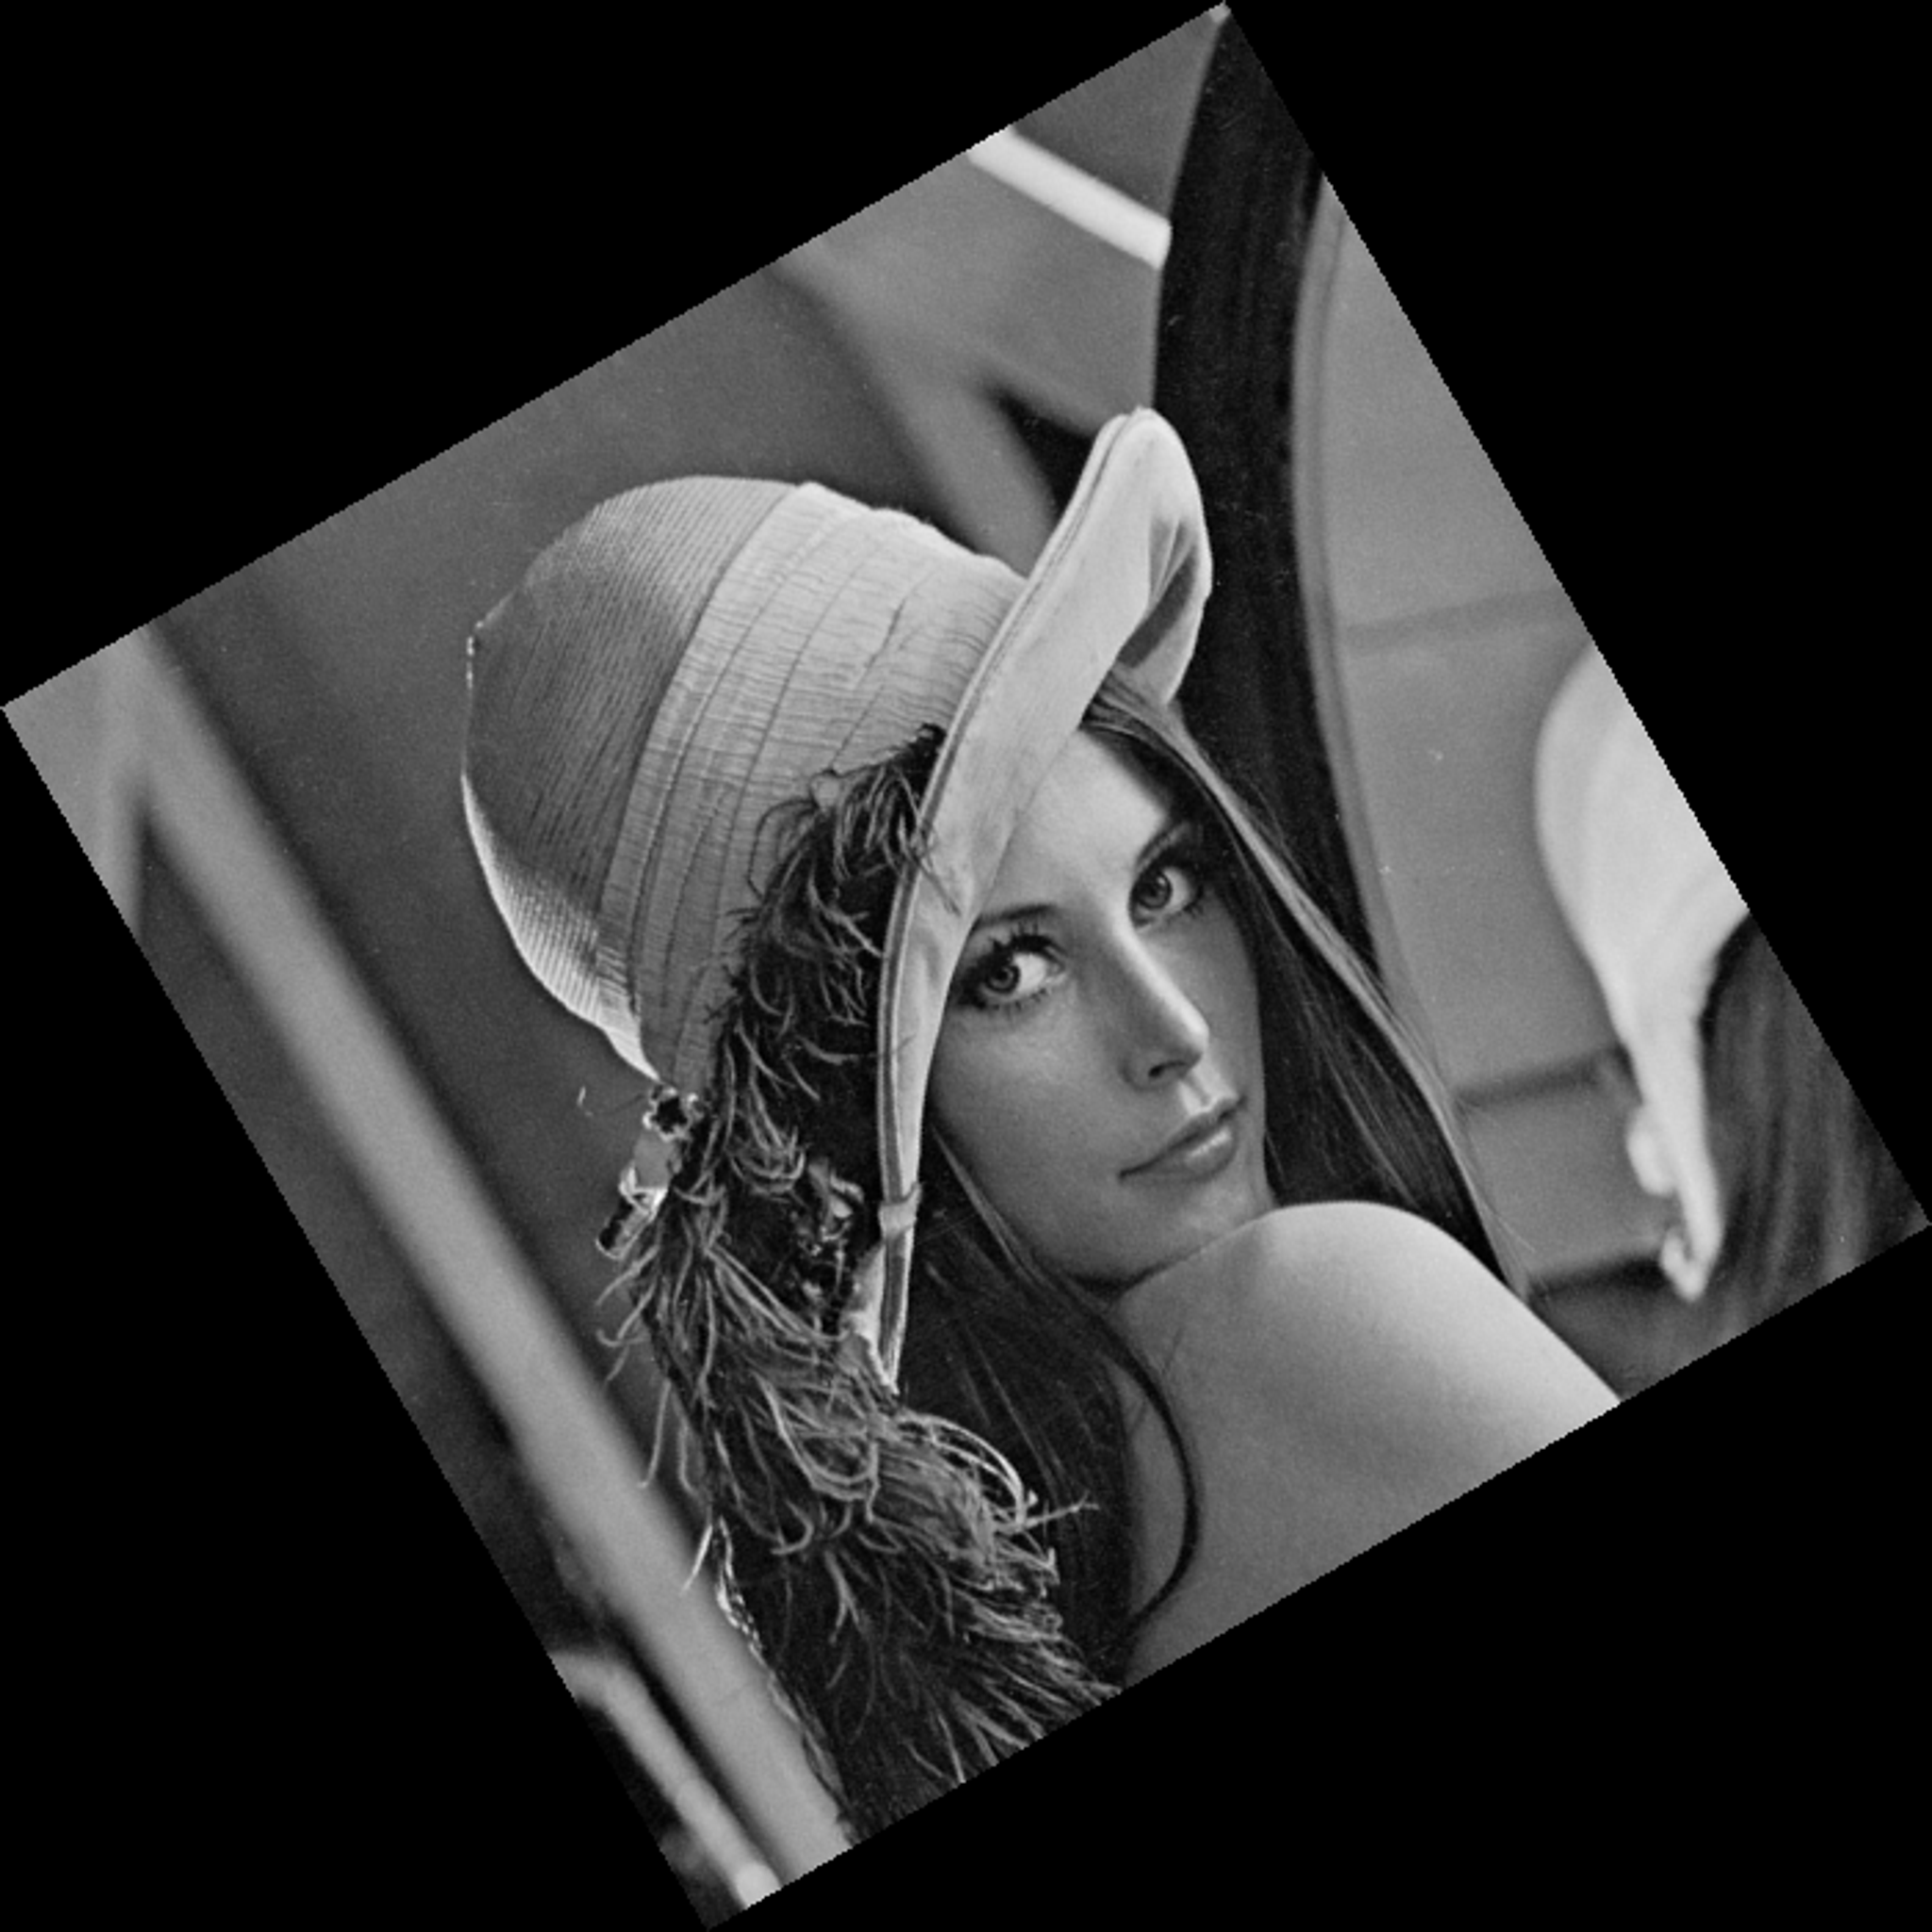
\includegraphics[width=\linewidth]{lena_rotate_30deg_2048_bicubic.png}
    \caption{Bicubic}
  \end{subfigure}
  \caption{Lena 旋转后三种插值放大对比}
\end{figure}

\subsubsection*{(4) Elain1：Shear 后插值放大}
\begin{figure}[H]
  \centering
  \begin{subfigure}{0.32\textwidth}
    \centering
    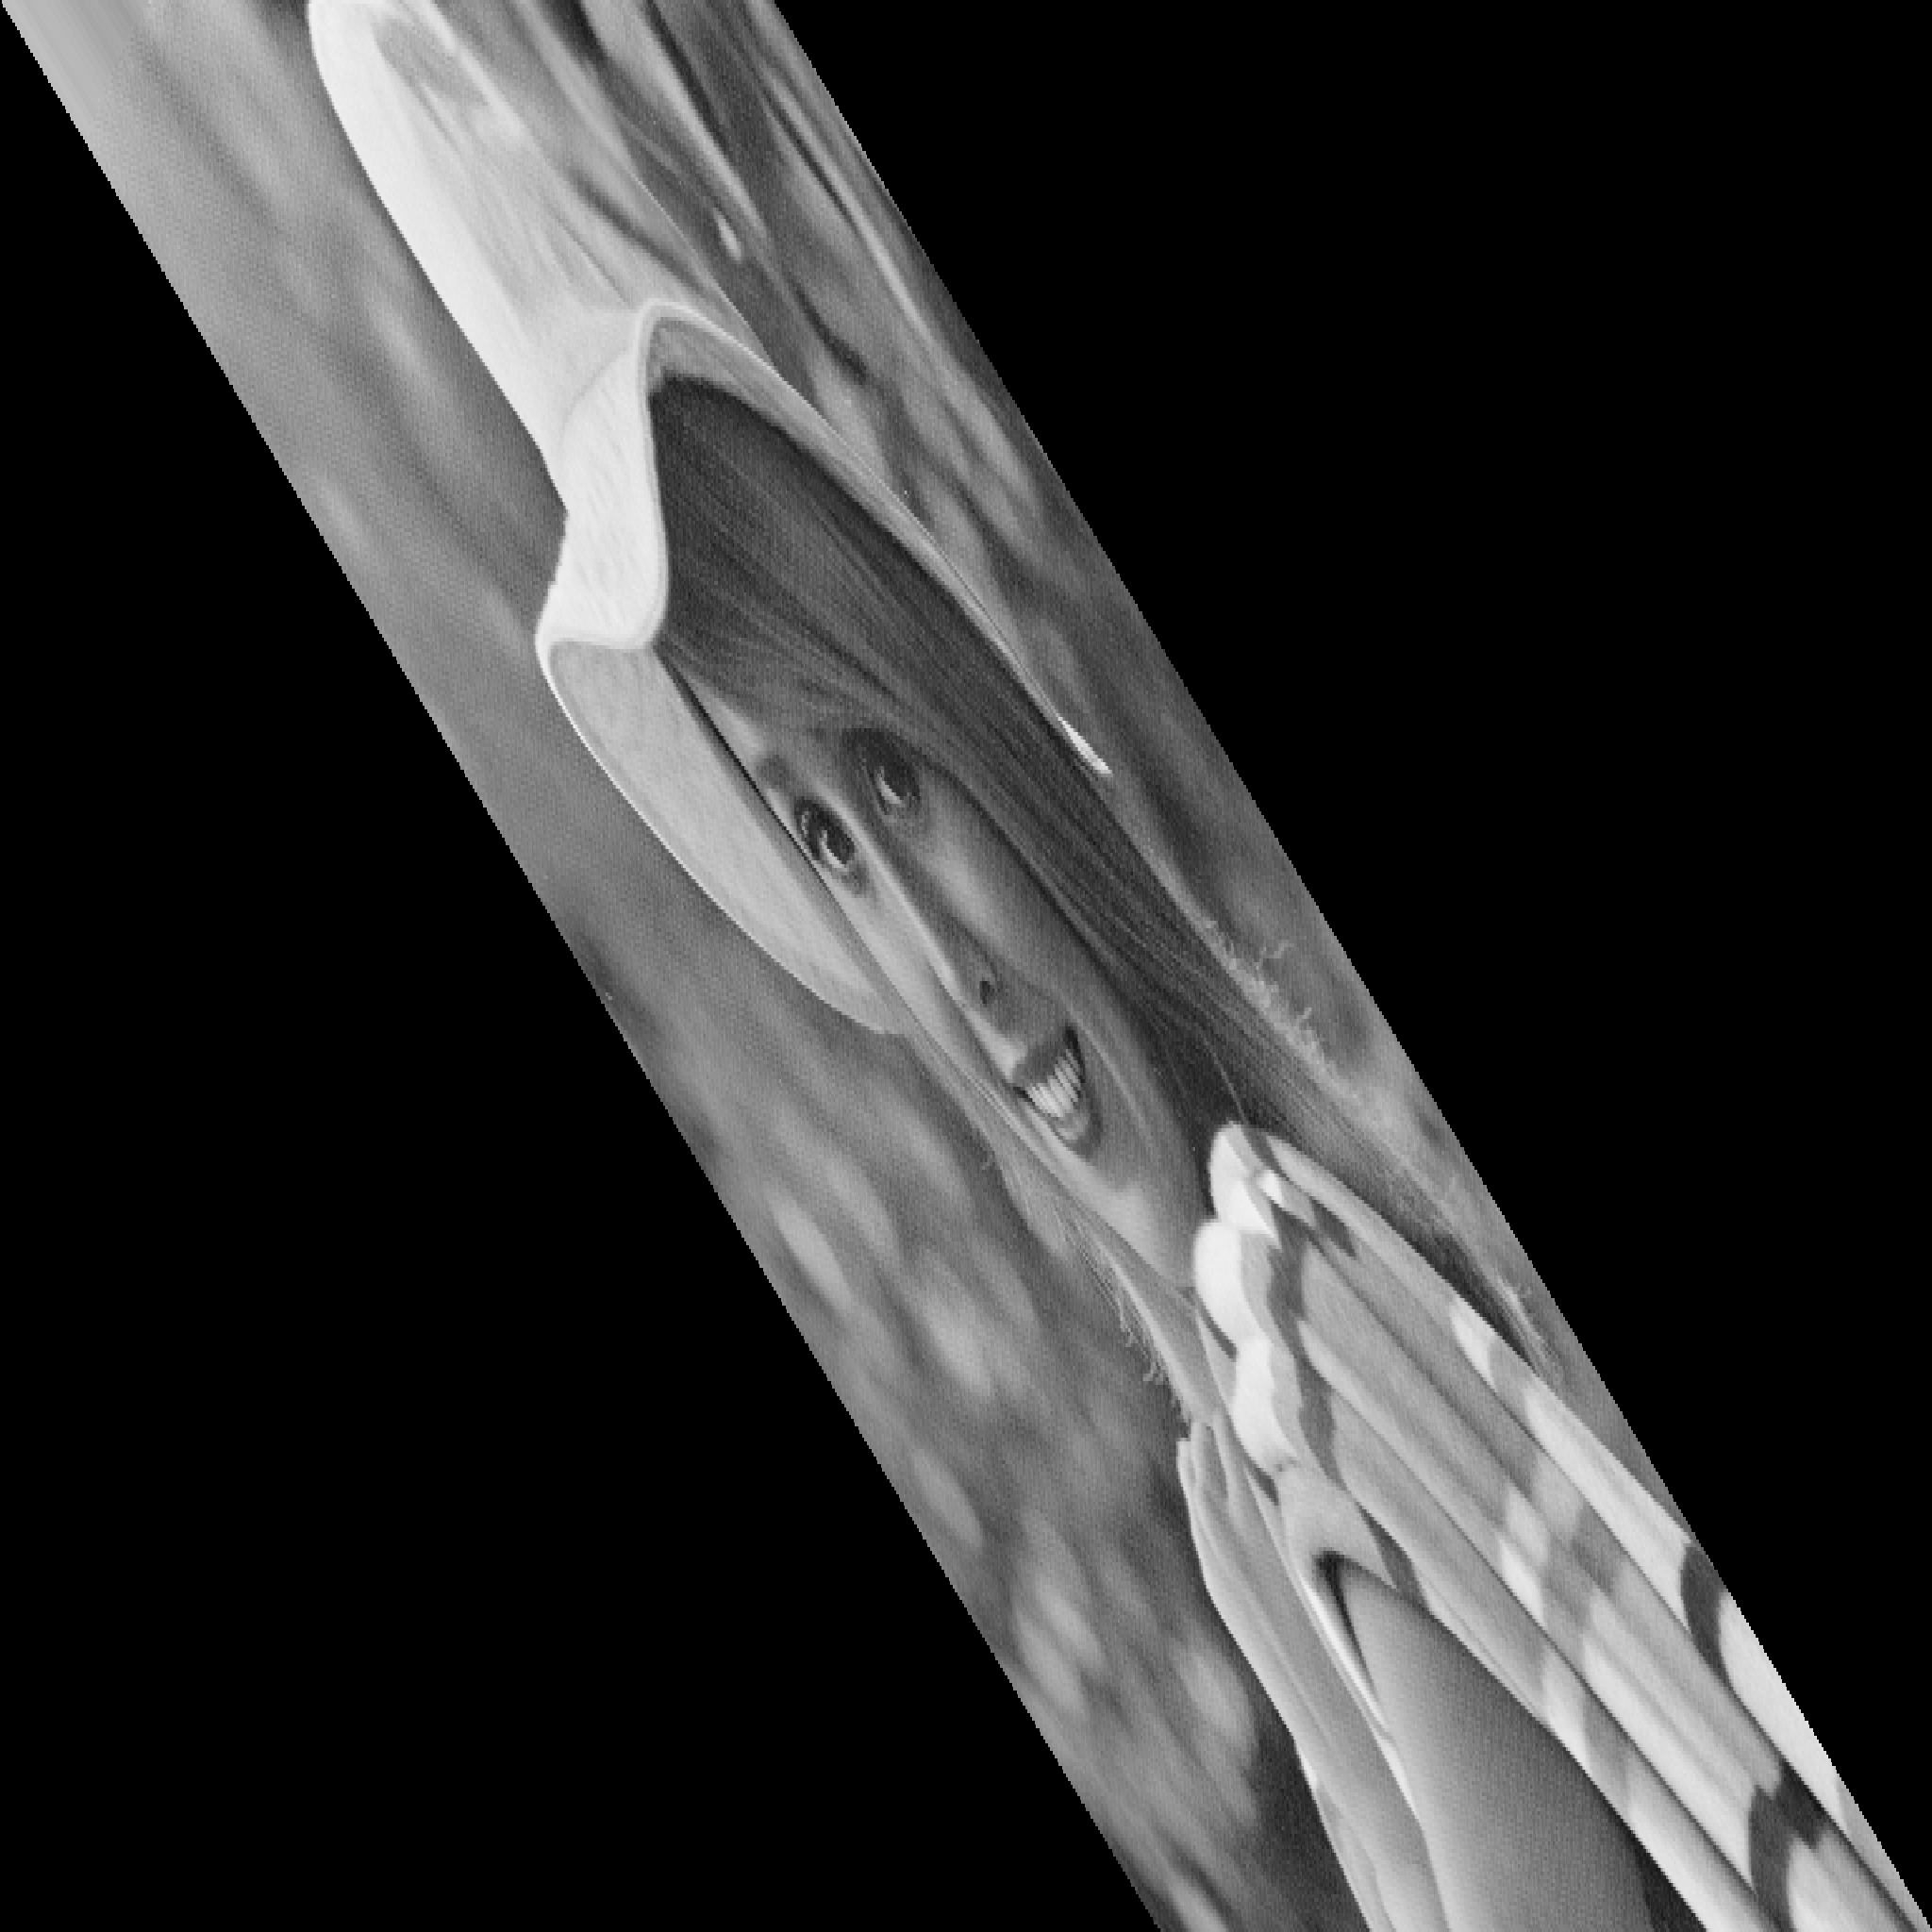
\includegraphics[width=\linewidth]{elain1_shear_k1.5_2048_nearest.png}
    \caption{Nearest}
  \end{subfigure}
  \begin{subfigure}{0.32\textwidth}
    \centering
    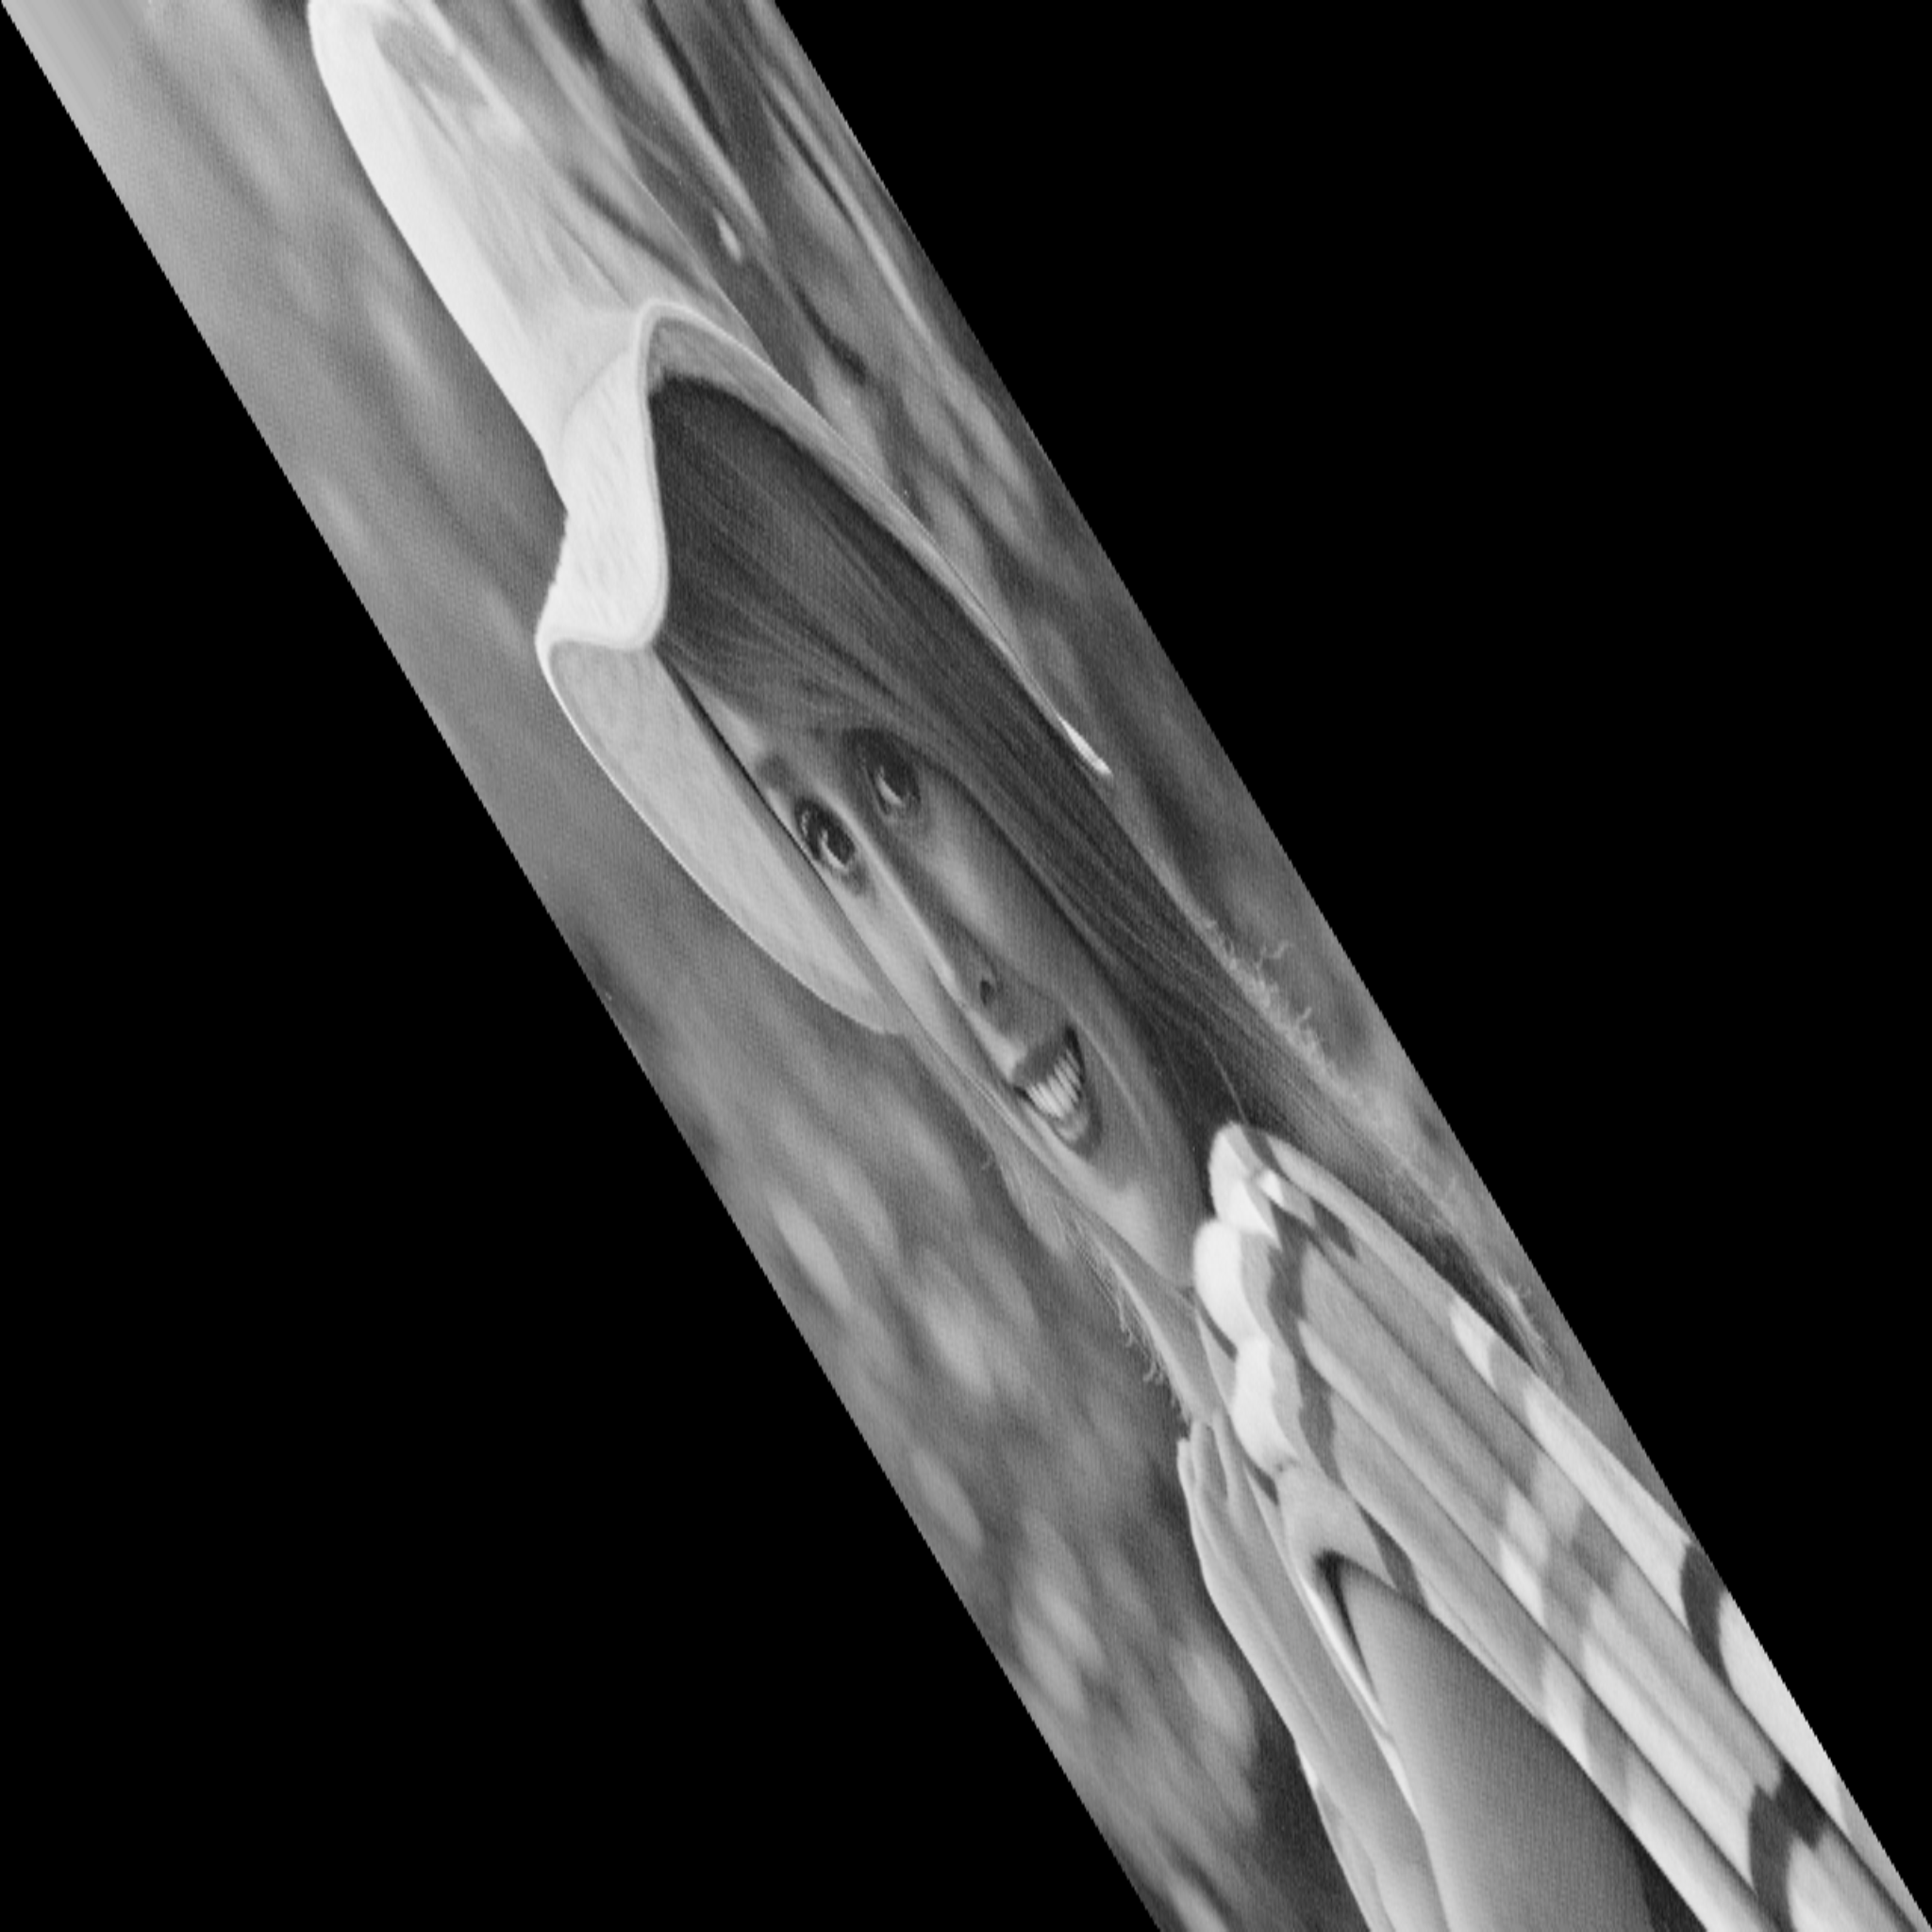
\includegraphics[width=\linewidth]{elain1_shear_k1.5_2048_bilinear.png}
    \caption{Bilinear}
  \end{subfigure}
  \begin{subfigure}{0.32\textwidth}
    \centering
    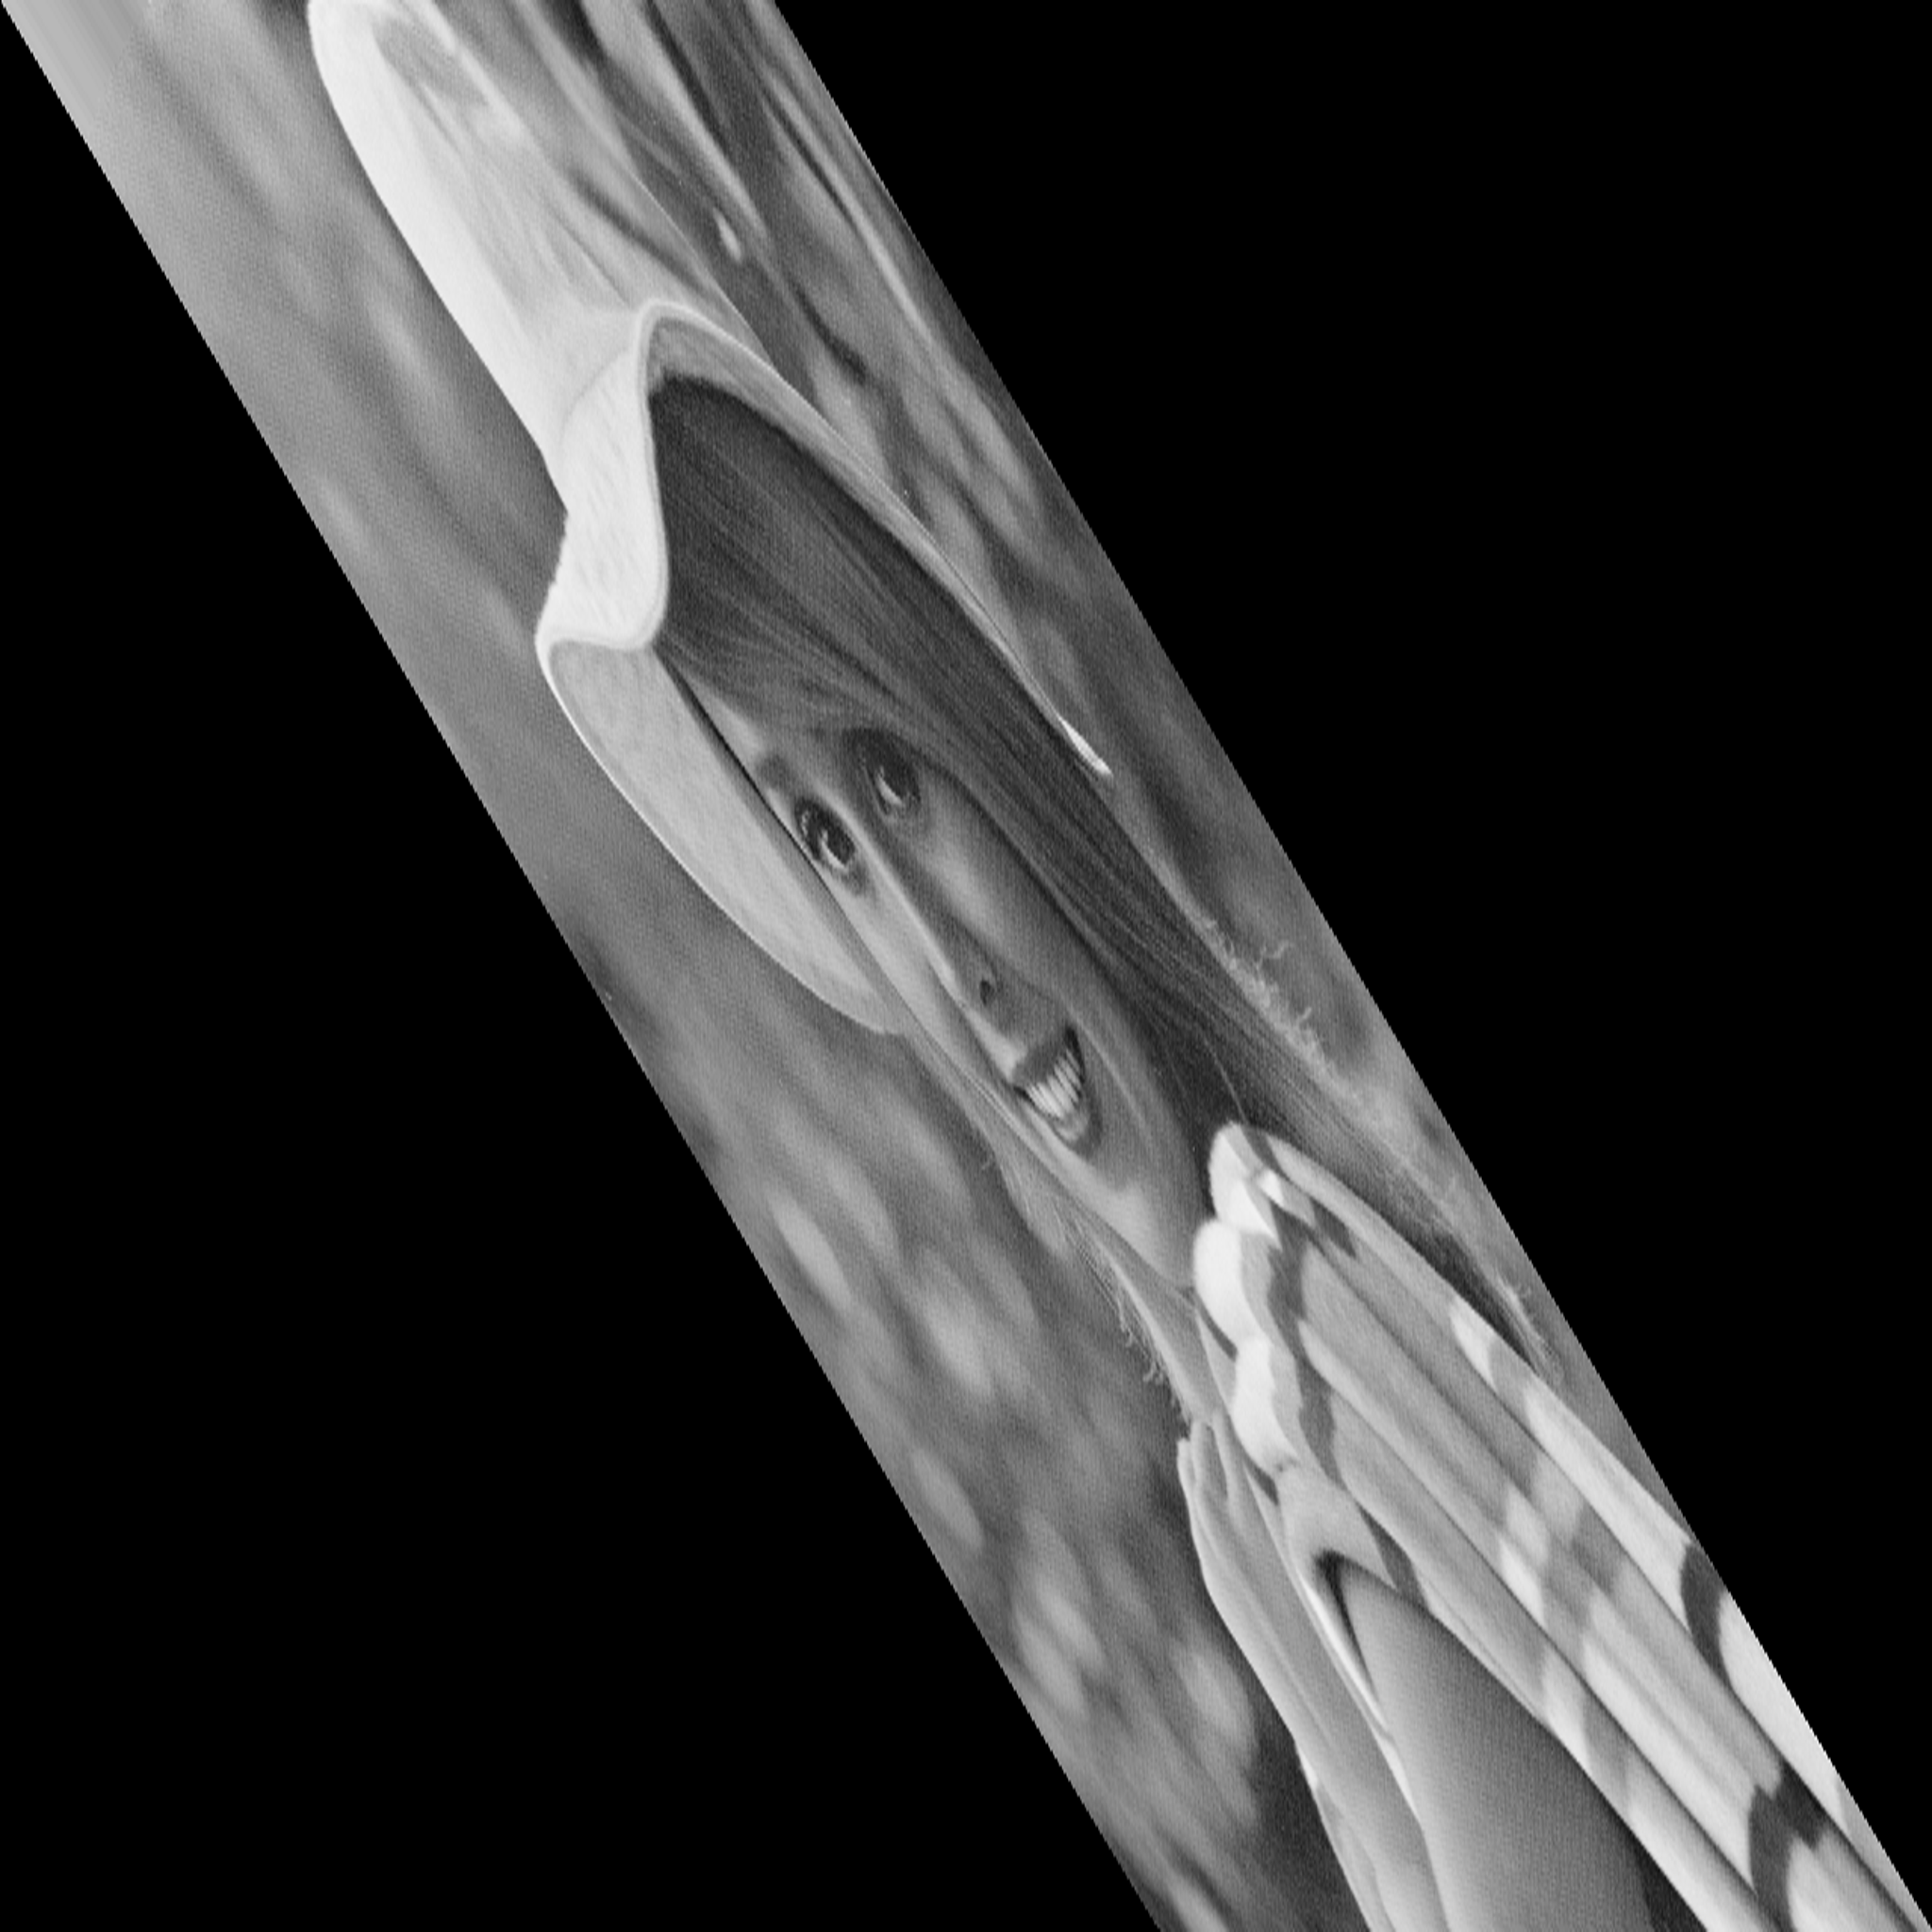
\includegraphics[width=\linewidth]{elain1_shear_k1.5_2048_bicubic.png}
    \caption{Bicubic}
  \end{subfigure}
  \caption{Elain1 Shear 后三种插值放大对比}
\end{figure}

\subsubsection*{(5) Elain1：旋转后插值放大}
\begin{figure}[H]
  \centering
  \begin{subfigure}{0.32\textwidth}
    \centering
    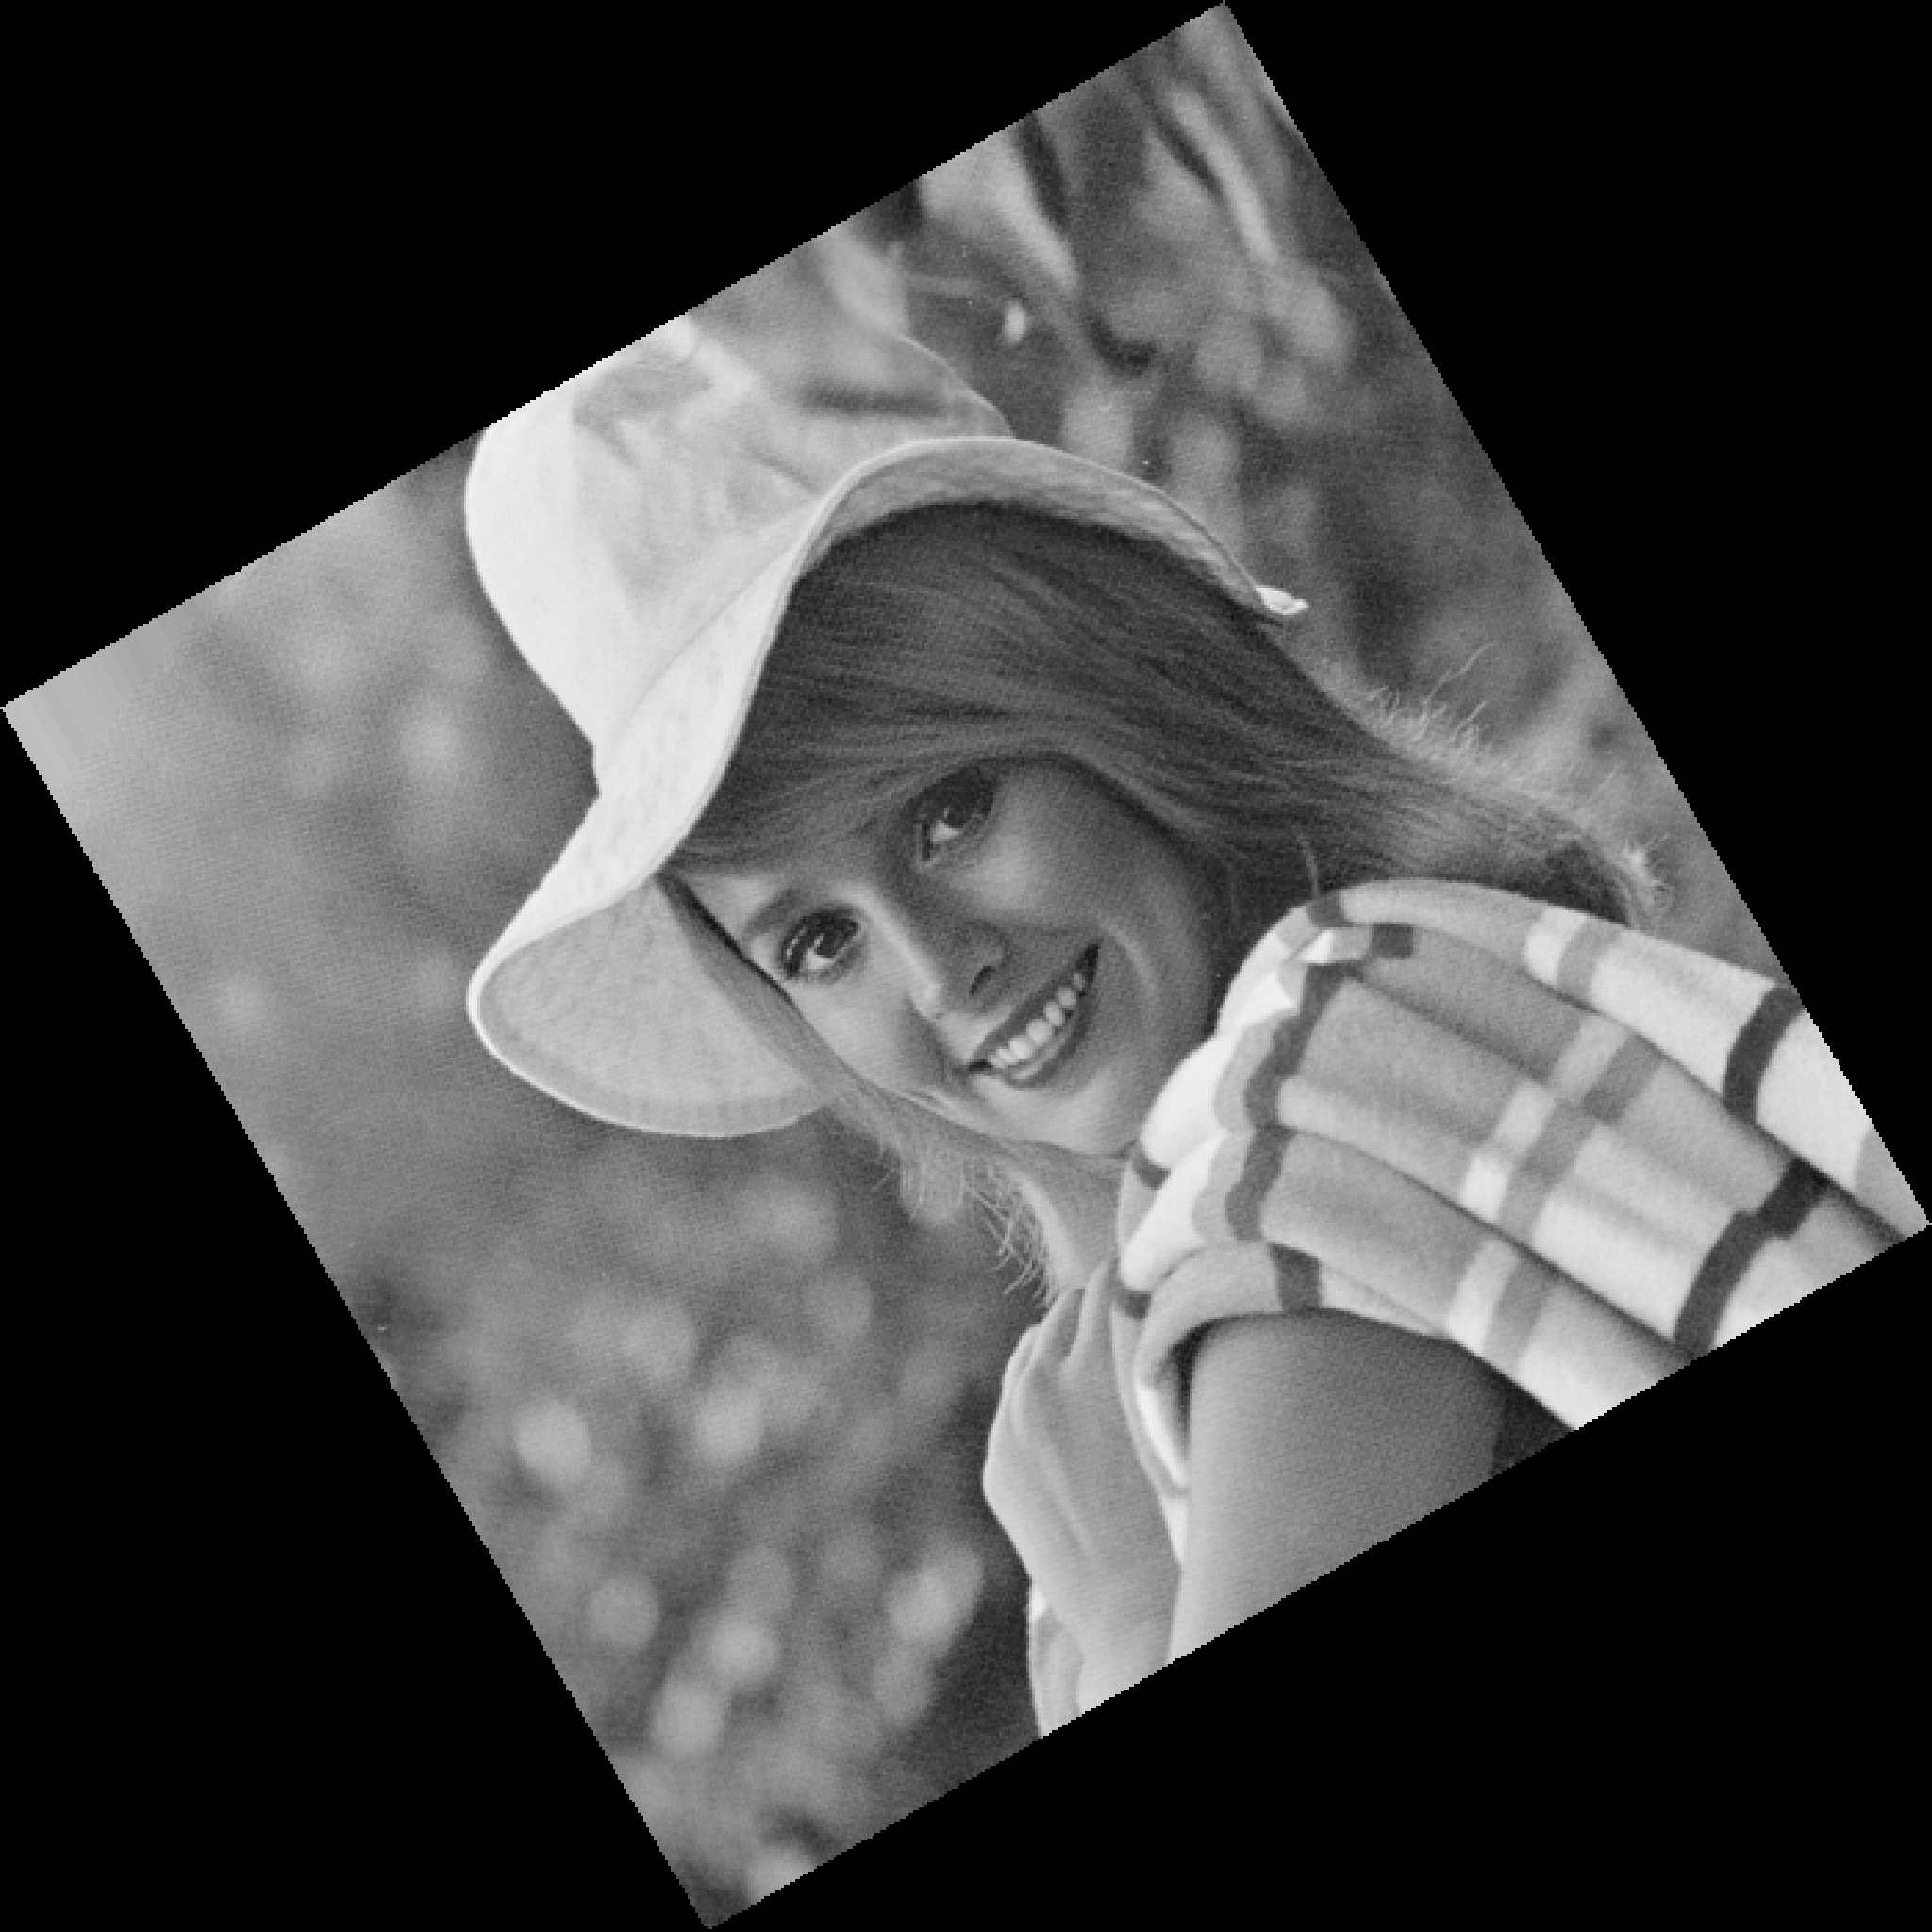
\includegraphics[width=\linewidth]{elain1_rotate_30deg_2048_nearest.png}
    \caption{Nearest}
  \end{subfigure}
  \begin{subfigure}{0.32\textwidth}
    \centering
    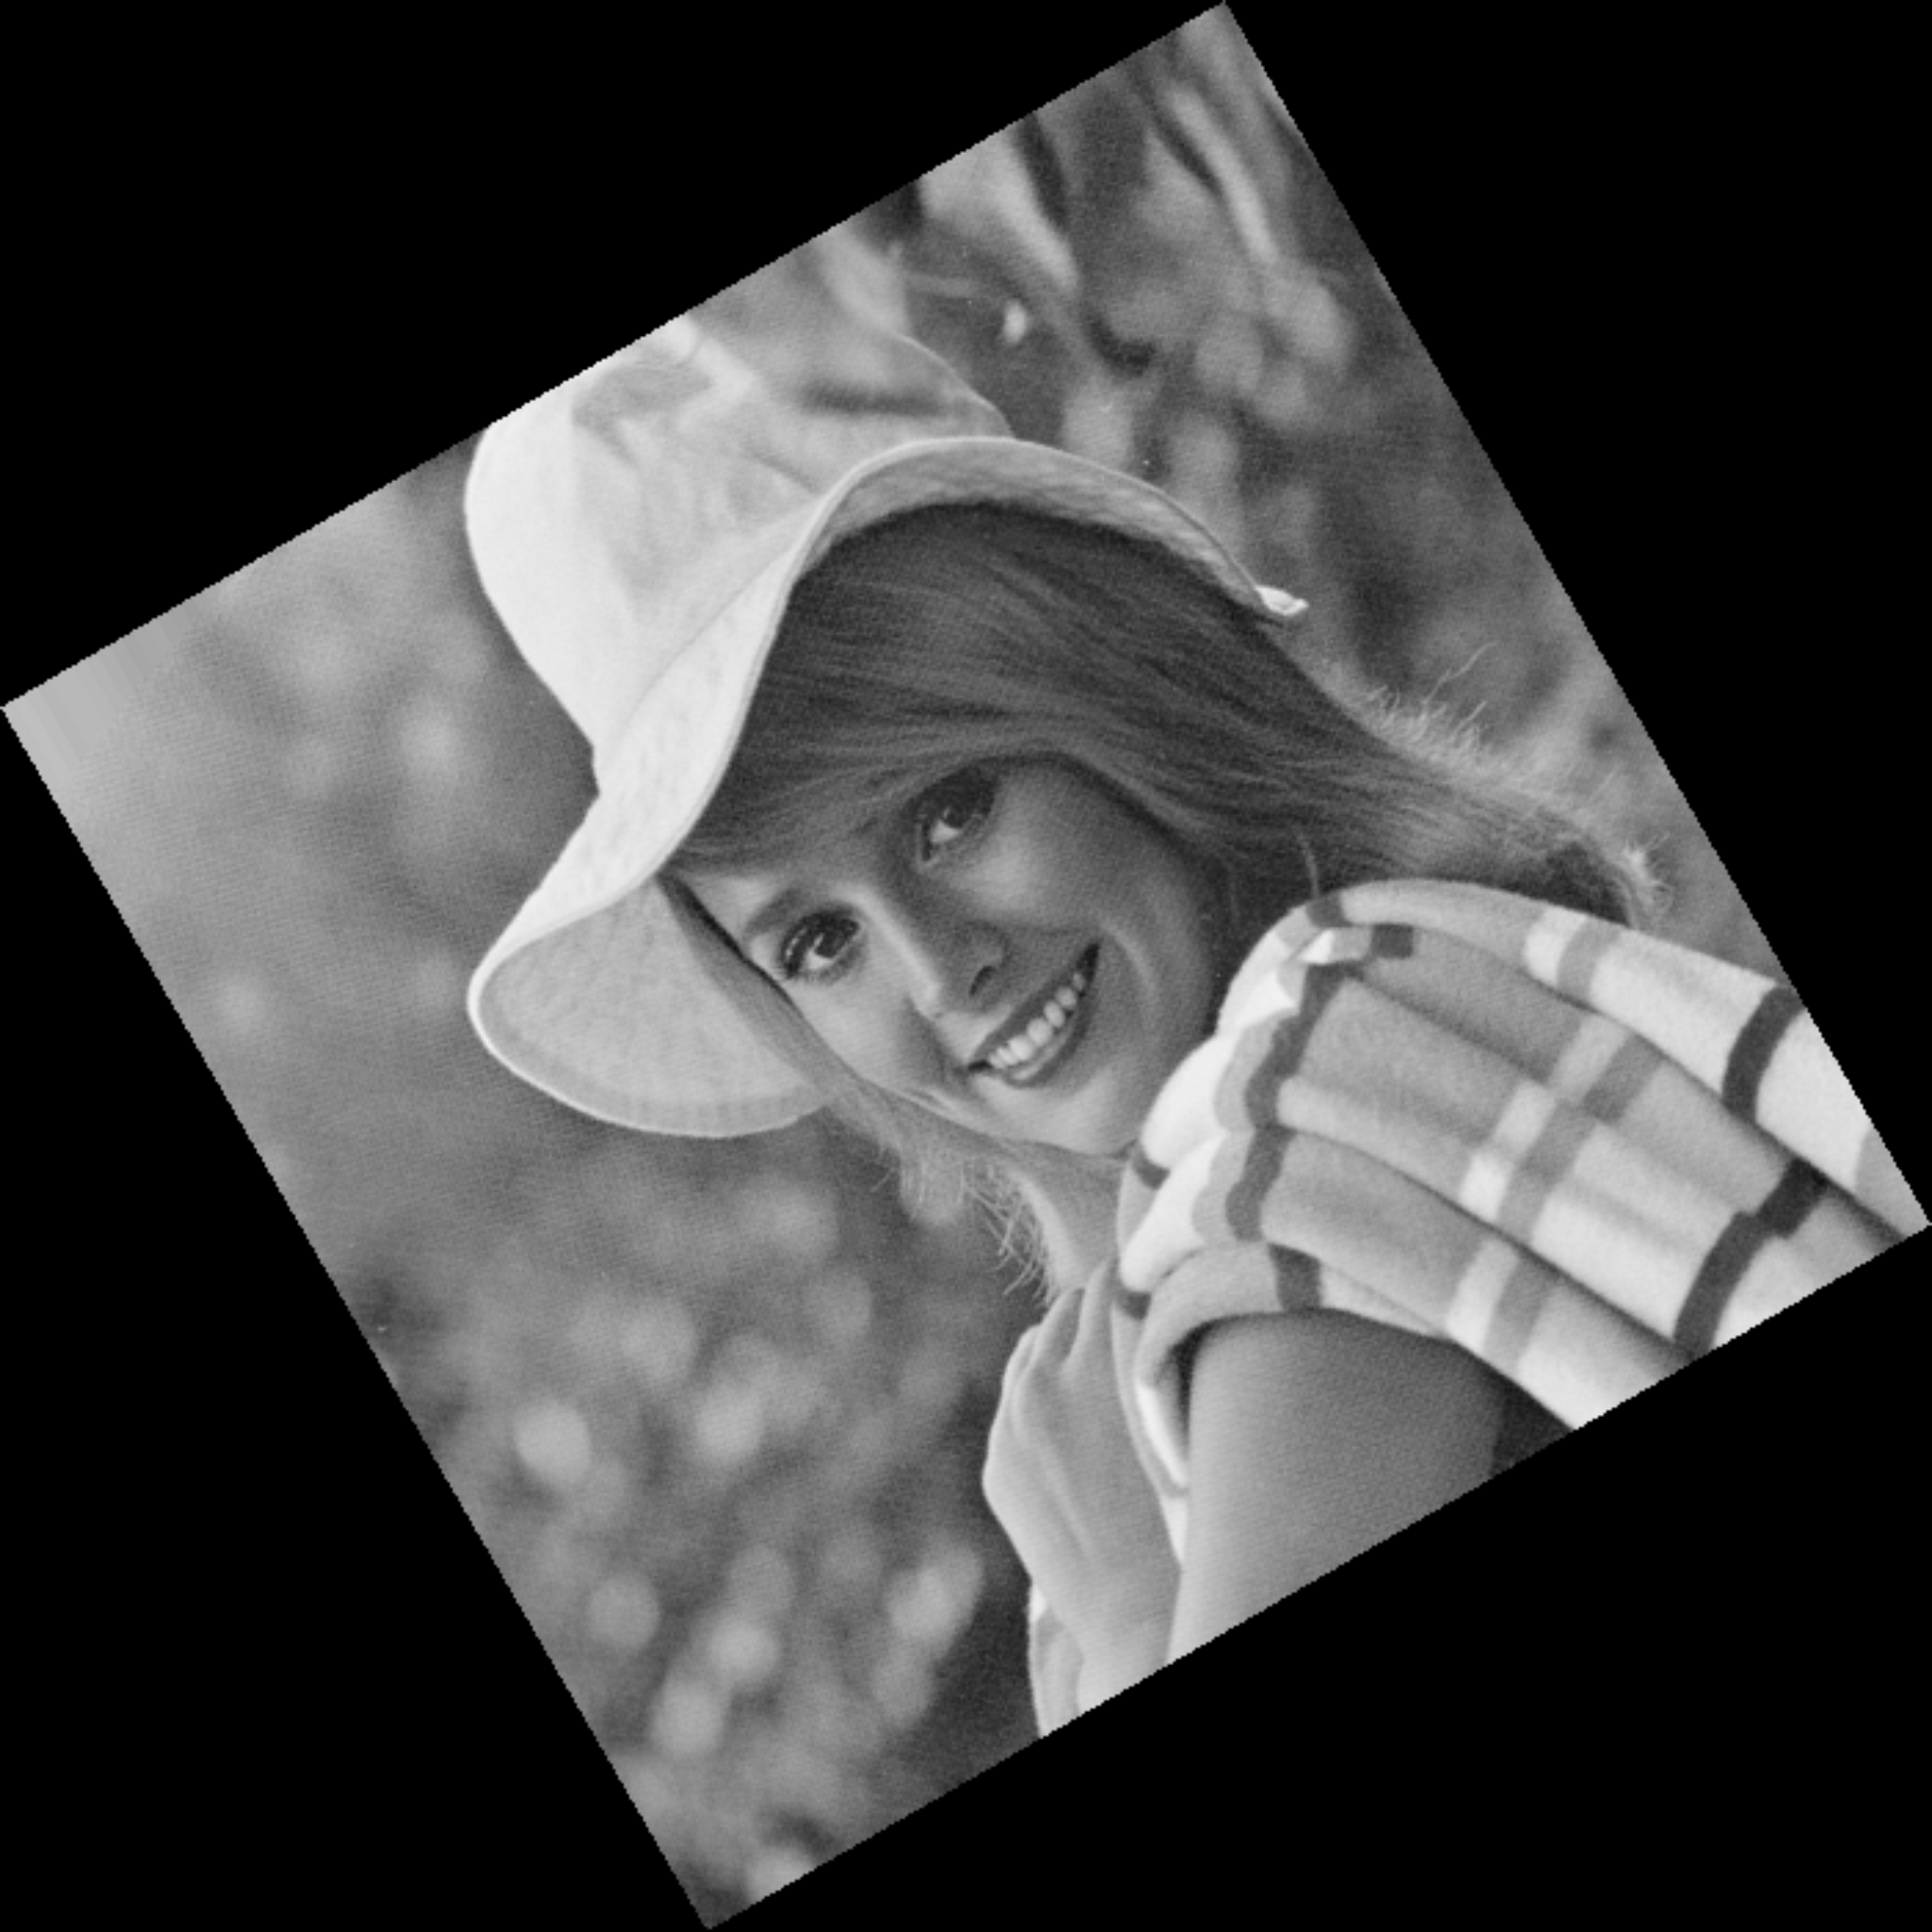
\includegraphics[width=\linewidth]{elain1_rotate_30deg_2048_bilinear.png}
    \caption{Bilinear}
  \end{subfigure}
  \begin{subfigure}{0.32\textwidth}
    \centering
    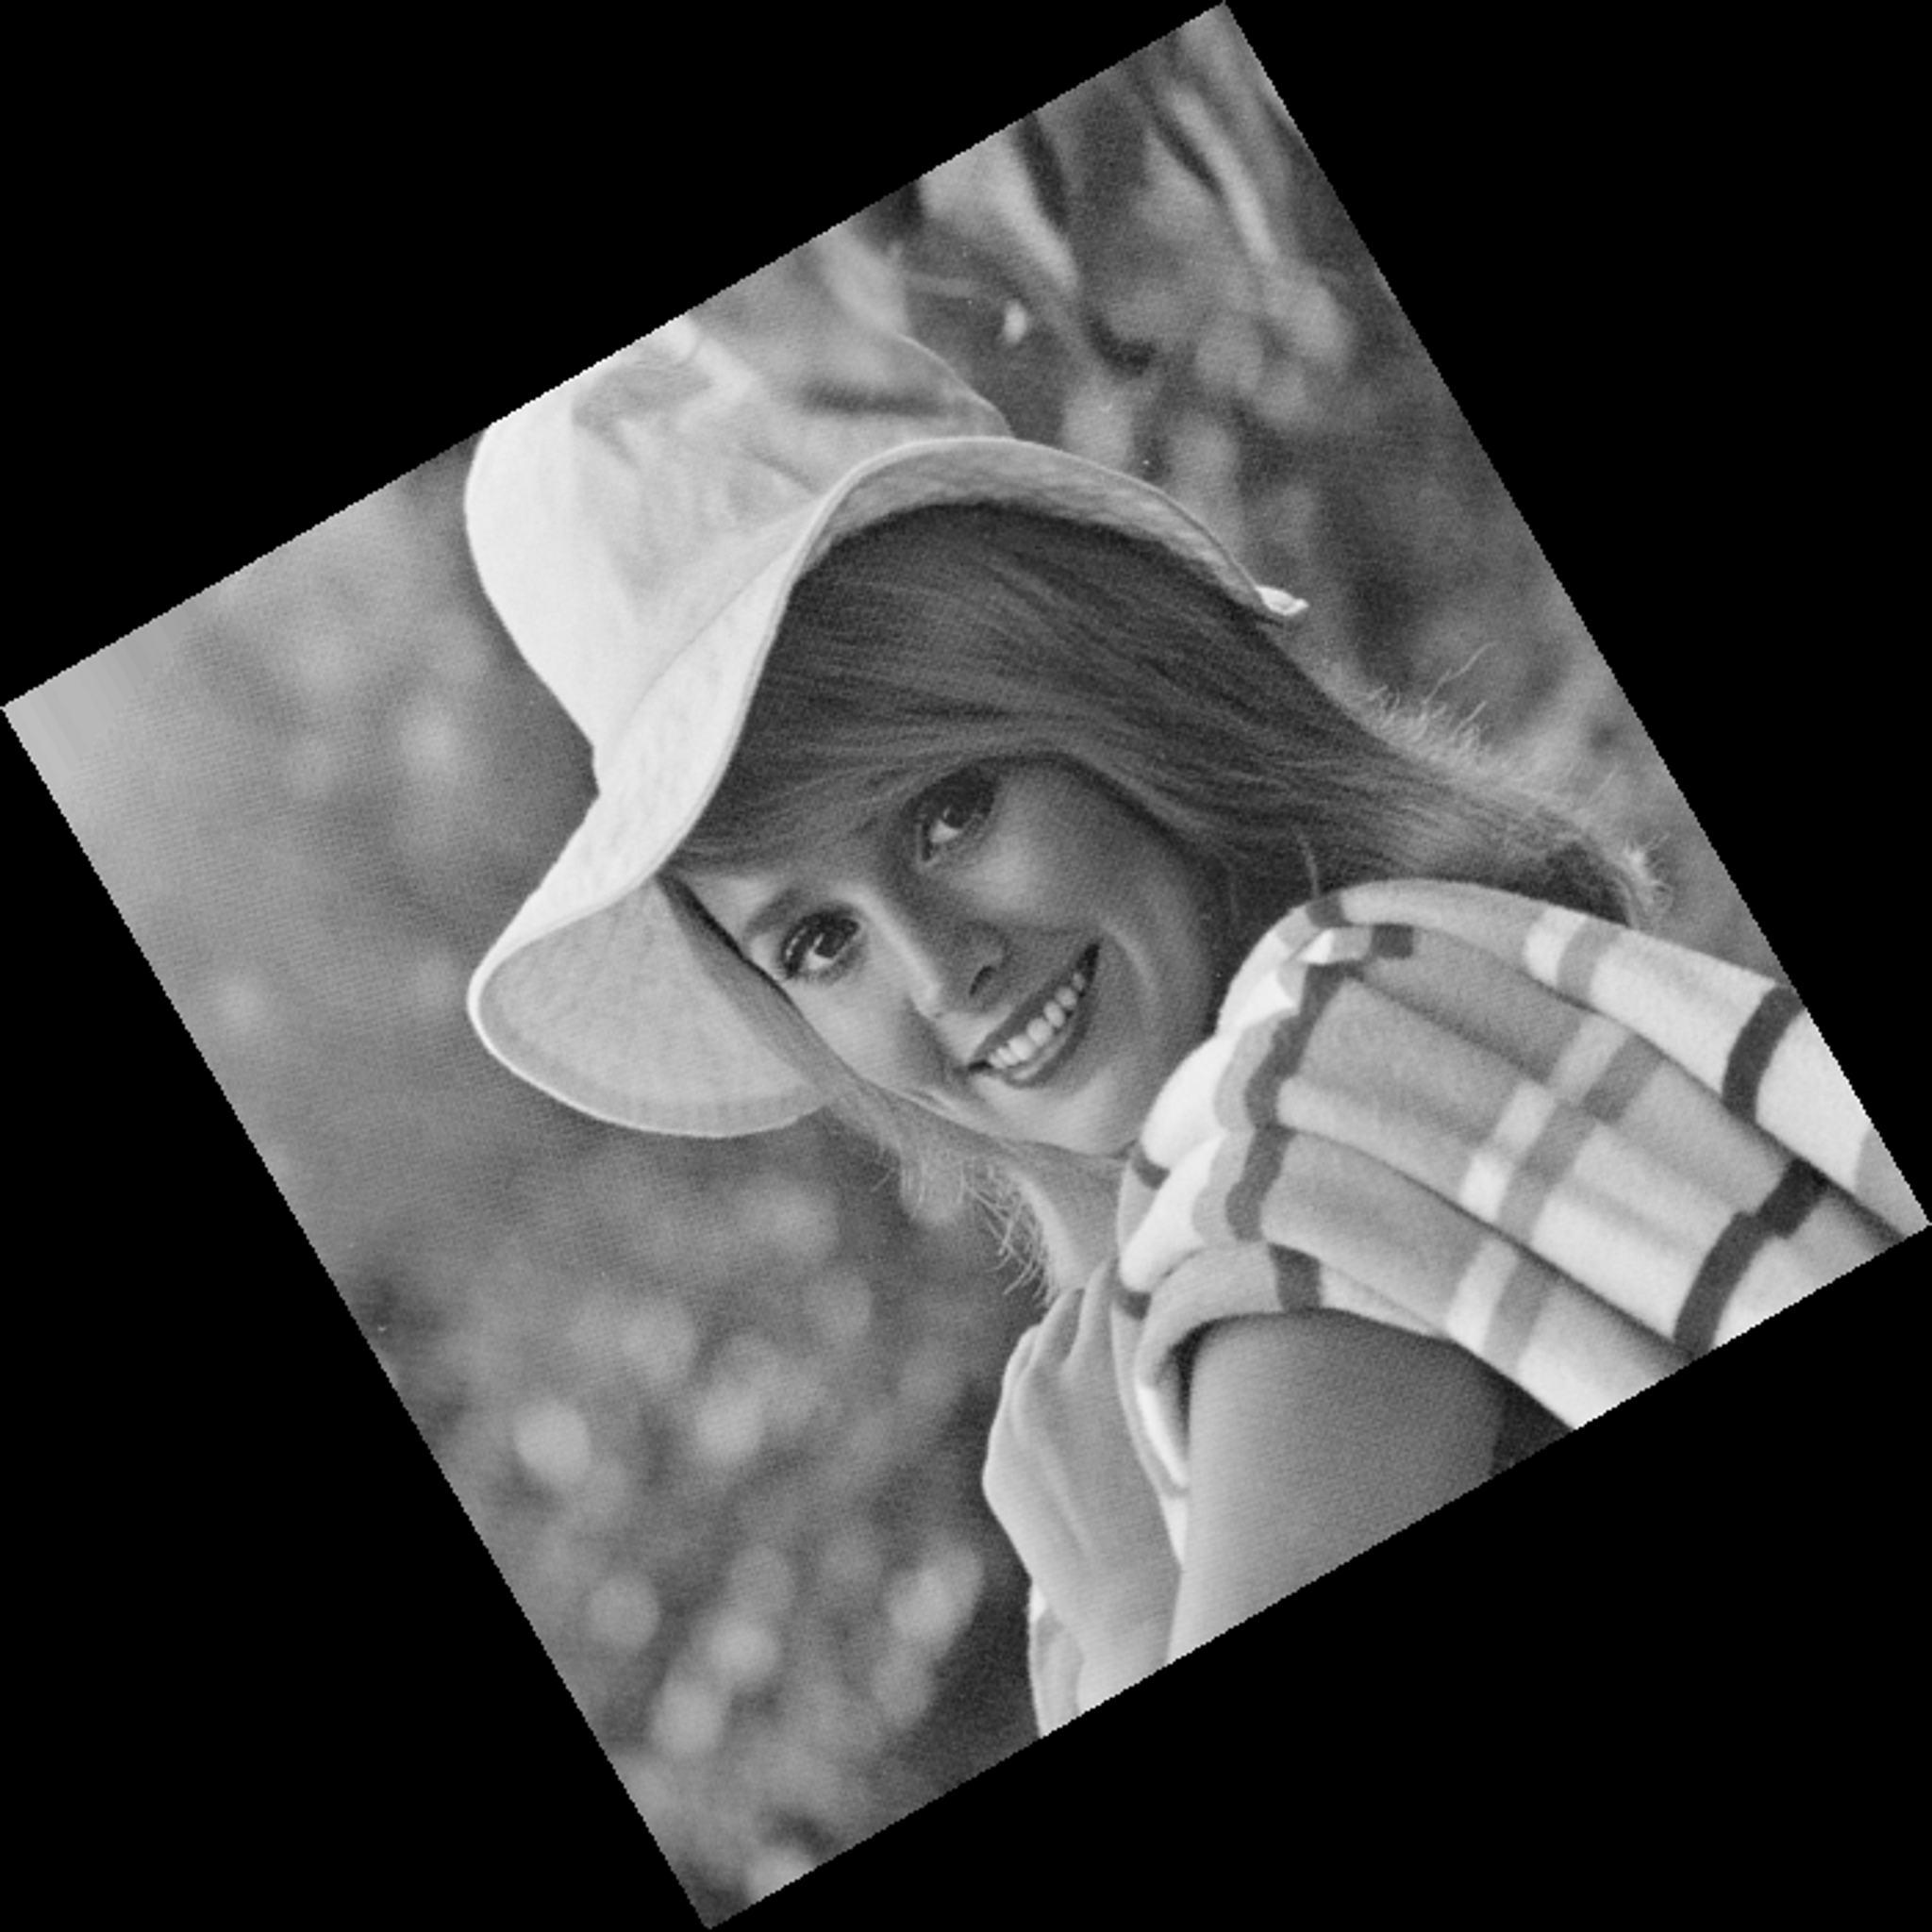
\includegraphics[width=\linewidth]{elain1_rotate_30deg_2048_bicubic.png}
    \caption{Bicubic}
  \end{subfigure}
  \caption{Elain1 旋转后三种插值放大对比}
\end{figure}

\section{结论}
\begin{enumerate}
  \item 通过解析 \texttt{7.bmp} 头部字段，验证了 BMP 的典型存储结构（文件头 + DIB 头 + 调色板 + 像素数据）。
  \item 灰度位深从 8 bit 降到 1 bit 时，图像细节逐渐丢失，伪轮廓逐渐增强。
  \item Lena 图像均值为 99.051216，方差为 2796.031839，说明图像整体偏中低灰且存在较明显亮暗层次。
  \item 在放大任务中，双三次插值在主观视觉质量上通常优于近邻与双线性。
  \item 几何变换后再放大时，插值方法差异更加明显，双三次在边缘连续性和细节保持方面表现更稳定。
\end{enumerate}

\section*{附：编译与使用说明}
\begin{itemize}
  \item 建议在 Overleaf 选择 \textbf{XeLaTeX} 编译器。
  \item 将本 \texttt{.tex} 文件与所有实验图片（含 \texttt{outputs/} 子目录）上传到同一工程。
  \item 若图片路径改变，只需修改导言区 \texttt{\textbackslash graphicspath} 配置。
\end{itemize}

\end{document}
